\section{Introduction}
\label{sec:intro-stamm}

Diverse biological processes have been observed to undergo transitions under influence of a stimulus. These transitions lead to changes on a cellular level between distinct phenotypic states. The source of these phenotypic changes can be morphological, epigenetic, or even at a protein interaction level.

One big obstacle in understanding the source of such phenotypic changes at a single cell level are that observations are gnerally not at the single cell level although it is only possible to perform observations on a population level. This restriction is experimental in nature and although sometimes it is possible to make observations on a single cell level there are limitations often on the amount of information that can be obtained as discussed in detail in Chapter \ref{cha:introduction}. 

The model we explore is called State transitions using aggregated Markov models (STAMM) initially proposed by \cite{Armond:2013}. This is a stochastic model identifying  state level information for single-cell transformations using population level data. Single-cell level dynamics, latent in the model, is described by a Markov chain which is then aggregated over multiple cells. Although this model has been applied to cancer cell lines as well \cite{Casale:2013} and stem cell reprogramming (see Chapter \ref{cha:stem-cells}) there is still work needed to obtain a better understanding of this model. We use single cell level simulations to probe model properties and model assumptions. 

A type of model that has found widespread application in the description and has shares certain characteristics with STAMM is the Hidden Markov model (HMM). Many examples of real world applications of HMMs exist including the deconvolution of population level microarray data \citep{Roy:2006ik}; some models also use simpler deconvolution algorithms for the cell cycle and for microarray data involving additional information \citep{Bar-Joseph04082004, BarJoseph:2008bx}. The main advantage of STAMM is that the latent model is in continuous time and therefore application to time-course data with uneven time-points is quite simple. This is discussed in more detail in Section \ref{cha:introduction}. Another type of model that is even closer to STAMM was studied by \cite{Kalbfleisch:1983vd} but this model investigates panel data and often near or at equilibrium. 

In this chapter we follow and expanding on the previous work done starting with a detailed description of STAMM Section \ref{sec:method} including a detailed description of model assumptions. In Section \ref{sec:estimation} we outline parameter estimation including a way to perform model selection as well as an efficient and unbiased estimation pipeline. Then we specify the single cell simulation setup (Section \ref{sec:sim-study})  before moving on to the results from single-cell simulation data in Section \ref{sec:results}. These are split up into results from performing a small scale simulation to probe the model and to test sensitivity to breaking assumptions; and large scale simulation results to demonstrate the whole pipeline.

\begin{figure}[!t]
  \centering
  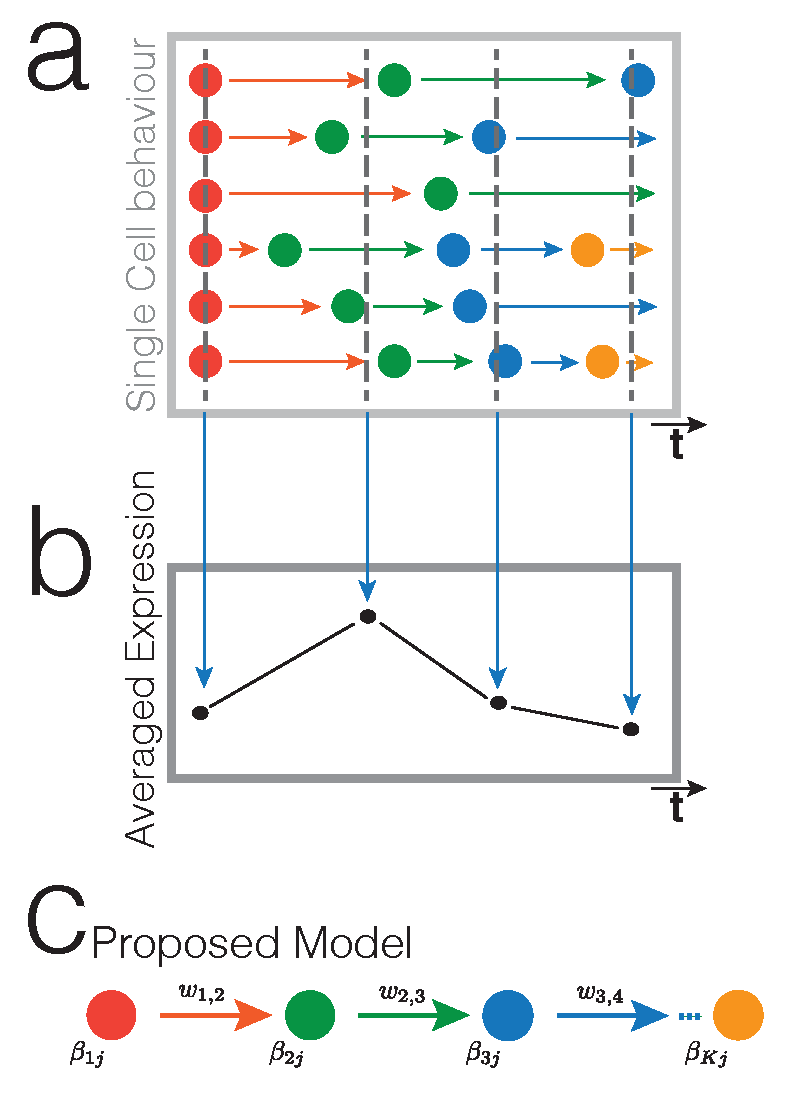
\includegraphics[width=0.6\textwidth]{pics/model_fig.pdf}
  \caption{Model description. (a) In any biological system undergoing transitions between multiple states where the time of transition is stochastic, cells states are heterogeneous in the population at any given time.  (b) Assays performed on homogenates of that cell population will only yield data averaged over sampled sub-populations. (c) We describe this system with 'State Transitions using Aggregated Markov Models' (STAMM) where single cell level processes are described by a latent continuous-time Markov chain which is aggregated over cells to give a likelihood (see Section \ref{sec:mast-model}). The Markov chain has a discrete state space which corresponds to biological states of the system (shown in different colours). Estimation of parameters in STAMM is performed using population level data. (Figure adapted from \cite{Armond:2013}.)  }
  \label{fig:model-sketch}
\end{figure}

\section{Model outline}
\label{sec:method}

\subsection{The STAMM model}
\label{sec:mast-model}


STAMM defines a latent stochastic process on the single cell level that isn't directly observed. Using the latent stochastic processes and aggregating across cells we can obtain a cell-population level likelihood. The latent single cell process is described using a Markov chain with a discrete and finite state space but it is continuous in time. Biological states in the system are identified with the state space, indexed by $k \in \lbrace 1, ..., K \rbrace$, is identified with biological states of the system. Transitions between states $k$ and $k'$ are determined by transition rates between these states denoted by $\mathbf{w} = \lbrace w_{k,k'} \rbrace $. Assuming that cell death and cell doubling compensate each other, i.e. the number of cells is conserved at all time $t$; the probability for any cell to be in state $k$ at any given time $t$ can be obtained by solving Master equation of the Markov chain. The resulting state occupation probability for the population $p_k(t;\mathbf{w})$ is a function of time and also the state transitions.

This model can fundamentally be applied to any type of time-course data, including transcript or protein abundance. Here unless otherwise stated we will focus the description, without loss of generality, on gene expression data. Let $x_j(t)$ be the cell-population-averaged gene expression of gene $j$ at time $t$, obtained from a homogenate assay such as RNA-seq or microarray expression. When investigating transitions it is prudent to design experiments with an initial state that is reasonably homogeneous, therefore our model assumes that initially all cells in the population occupy the same state, this is often part of the experimental design of investigating changes from an initial homogeneous starting population. At any subsequent time point cells exist in a mixture of states, hence any measurement $x_j(t)$ made on a population level is an average over multiple states. We further assume that there is a mean expression level per gene constant across a state. This is denoted by $\beta_{kj}$, the gene expression level for gene $j \in \lbrace 1 \ldots p \rbrace$ in state $k$.

In the limit of large numbers of cells the fraction of cells in any state $k$ is given by the state occupation probability $p_k(t;\mathbf{w})$. We can now write the observed average gene expression, $x_j(t)$ for gene $j$ at time $t$, as the sum of all occupation probabilities weighted by their respective gene expression signatures. The resulting model for the average gene expression from a latent Markov chain model is written as:

\begin{equation}
  x_j(t) = \sum_k p_k(t;\mathbf{w})\beta_{kj} = P(t;\mathbf{w}) \, \beta_j,
  \label{eq:model}
\end{equation}
where the right hand side is the vectorized form of the model, with the row vector $P(t;\mathbf{w}) = [p_1(t,\mathbf{w}), \ldots , p_K(t,\mathbf{w})]$ and column vector $\beta_j = [\beta_{1j}, \ldots , \beta_{Kj}]^T$. Assuming an additive Gaussian noise model with gene-specific noise variance $\sigma_j^2 $ we arrive at the likelihood:

\begin{equation}
  \label{eq:likelihood}
    \mathcal{L} \left(\mathbf{w}, \beta_j, \sigma_j \;|\; \lbrace x_j(t)\rbrace\right) = 
\prod_{t=1}^T \mathcal{N}\left(g(x_j(t)) | g\left(P(t; \mathbf{w})\,\beta_j\right),\; \sigma_j^2 \right),
\end{equation}
where $\mathcal{N}(\cdot | \mu,\sigma^2)$ denotes a Normal density with mean $\mu$ and variance $\sigma^2$ and the function $g$ denotes a transformation whose choice depends on the data type under investigation.

Applied to microarray experiment which use ratios of fluorescence intensities between measurements in the red spectrum $R$ and green spectrum $G$. The transformation $g$ used is $\log_2$ \cite{Dudoit:2002va}, for further details see Section \ref{sec:microarray}. When investigating RNA-seq data we use $\arcsinh$ as the transformation \citep{Hoffman:2012gn,Johnson:1949uq}, defined as $\arcsinh(x) = \ln(x + \sqrt(x^2 +1))$ (for more details see Section \ref{sec:norm-stand}). RNA-seq data cannot be normalised in the same way as microarray data most importantly because it contains measurements which are exactly zero. The $\arcsinh$ normalisation is useful here, because unlike the log transformation it does not have a singularity at zero but has the same variance-normalisation properties.

To use the likelihood it is necessary to compute the state occupation probabilities at any time $t$ observations are made.
% We discuss below how to compute these from latent Markov chain process.

\subsubsection{Markov chain and the master equation}
\label{sec:markov-chain-master}

Until now we have not placed any restrictions on the latent Markov process in this model and we have formulated the
likelihood eqn. (\ref{eq:likelihood}) for a general case. If we let the states be $k \in \lvert 1 \ldots K \rvert$ and denote transitions between states $k$ and $k'$ as $\mathbf{w} = \lvert w_{k,k'} \rvert$. 
% TODO finalise paragraph
The topology of the Markov chain has implication on identifiability of the model (further discussion Section \ref{sec:identifiability}). Here we limit ourselves to a pure birth process where $w_{k,k+1} \ne 0$ for all $k$ and zero otherwise. Such a Markov chain also excludes branches. The resulting master equation is written as:
\begin{equation}
  \label{eq:master}
  \frac{d p_k(t)}{dt} = w_{k-1,k}\, p_{k-1}(t) - w_{k,k+1}\, p_k(t).
\end{equation}

To simplify further calculations the master equation is rewritten in matrix notation. Let $\mathbf{G}(\mathbf{w})$ be a $K \times K$ matrix whose only non-zero entries are on the diagonal, $g_{kk}=-w_{k,k+1}$, and the subdiagonal $ g_{k\,k-1}=w_{k-1,k}$. Now we can write the solution to the master equation as
\begin{eqnarray}
  \label{eq:masterMat}
  P(t; \mathbf{w}) &=& \exp{\left(\mathbf{G}(\mathbf{w})\,t \right) } {P}(0)
\end{eqnarray} 
In investigating transition processes (such as Chapters \ref{cha:oncog-transf}, \ref{cha:stem-cells}) in general an experimental design is chosen such that the initial cell population is in the same state. Therefore we can set the initial conditions for the state occupation probability, $P(0) = (1, 0 , 0, \ldots)$. This means all cells are in state $k=1$ at $t=0$ just before the cell population is perturbed. This allows us to write the closed form solution for the state occupation probability as:
\begin{eqnarray}
  \label{eq:state-occ}
  P(t; \mathbf{w}) &= & \exp{\left(\mathbf{G}(\mathbf{w})\,t \right) } {P}(0).
\end{eqnarray}

This expression is also used to evaluate the likelihood (equation (\ref{eq:likelihood})) of the model for different parameters.

\subsubsection{Model Assumptions}
\label{sec:model-assumptions}

We make a number of assumptions in the above model derivation. Here, we focus on some of the key assumptions made regarding the transition process on a single cell level and investigate them further. Ensuring an analytically tractable latent state change model makes these assumptions necessary. In the discussion below we discuss how legitimate these assumptions are, if and how they can be relaxed and how they can be justified.

First, we assume expression of a gene remains constant while it remains inside a given state. The single cell expression of each gene is modeled by a piecewise flat trajectory where expression changes are instantaneous due to a change in state. It also has the effect that the only time-dependence in the likelihood is due to the state occupation probabilities of the Markov chain. In this simple approximation, interaction between genes are ignored; allowing us to formulate a computationally efficient pipeline to estimate parameters for time courses with many genes, see Section \ref{sec:estim-pipe} for further details. It is a very strong assumption and apart from the noise that is prevalent in most biological systems gene expression also changes inside a state due to cell internal mechanisms e.g. the cell-cycle. The slightly more relaxed but sufficient assumption here is: Temporal changes within a state should be much smaller than the difference between biologically distinct states for genes influential in such a transition. This case is illustrated in Figure \ref{fig:influential-schematic} and \ref{fig:influential1-schematic}. Therefore this is still a good first approximation in the case of transition processes. 

\begin{figure}
  \centering
  \subfigure[Influential gene]{
    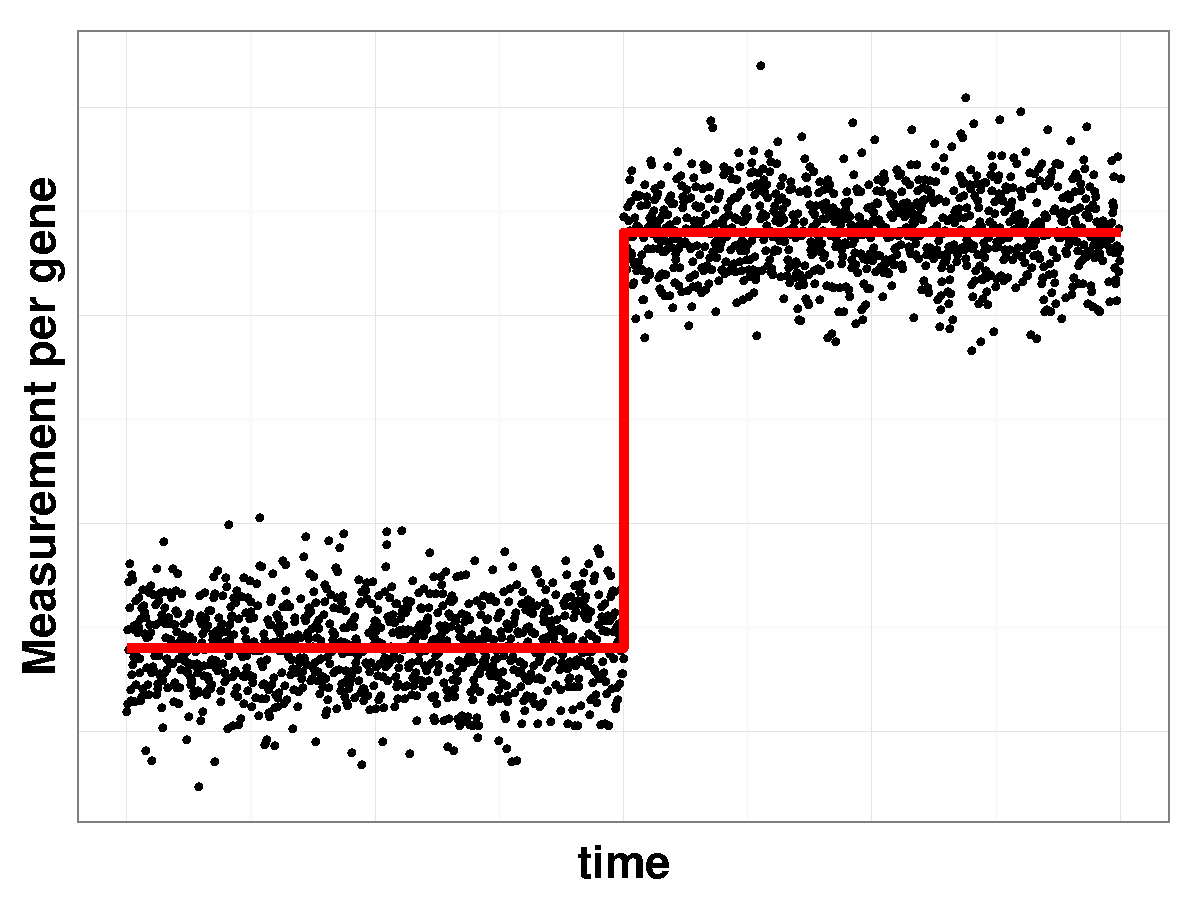
\includegraphics[width=0.45\textwidth]{pics/assmptn11.pdf} \label{fig:influential-schematic}
  }
  \subfigure[Influential gene gradual change]{
    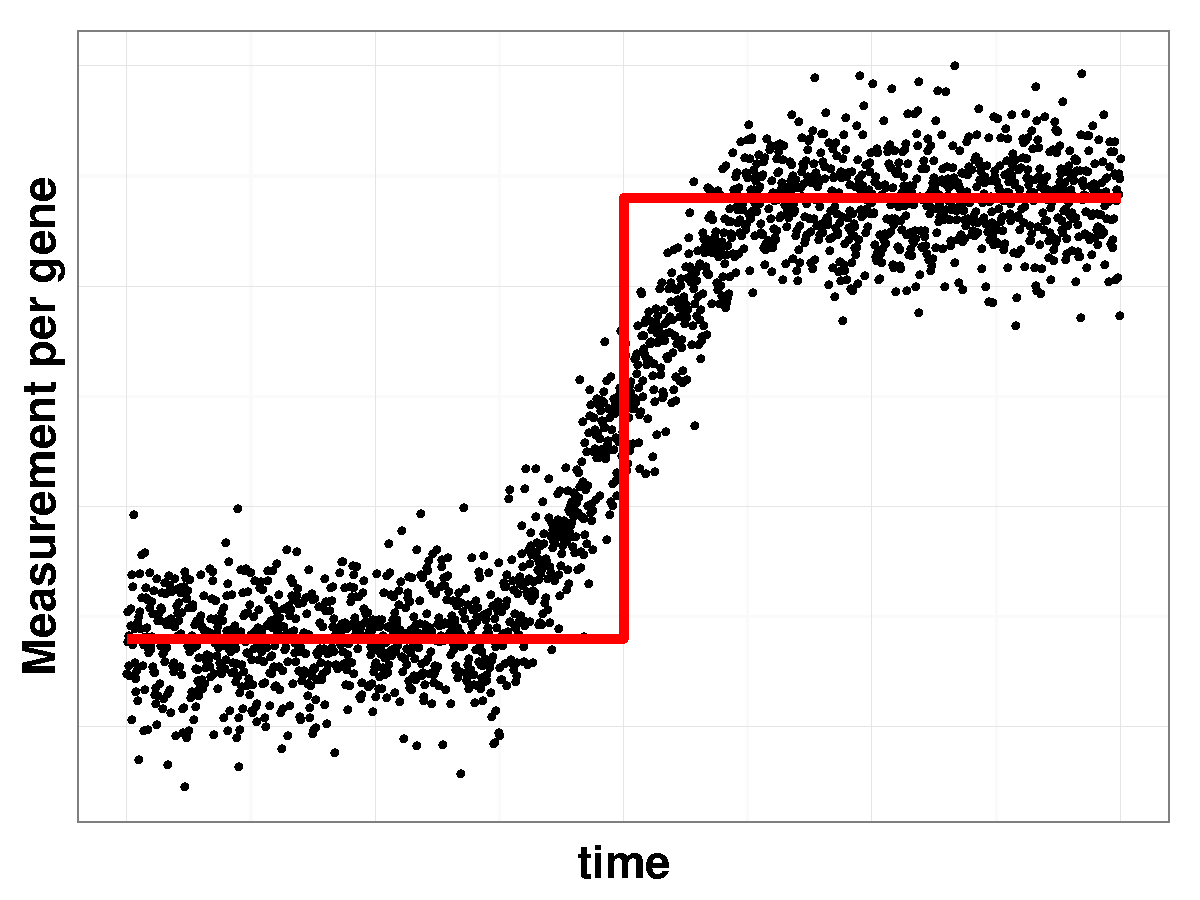
\includegraphics[width=0.45\textwidth]{pics/assmptn12.pdf} \label{fig:influential1-schematic}
  }
  \subfigure[Gene not influential]{
    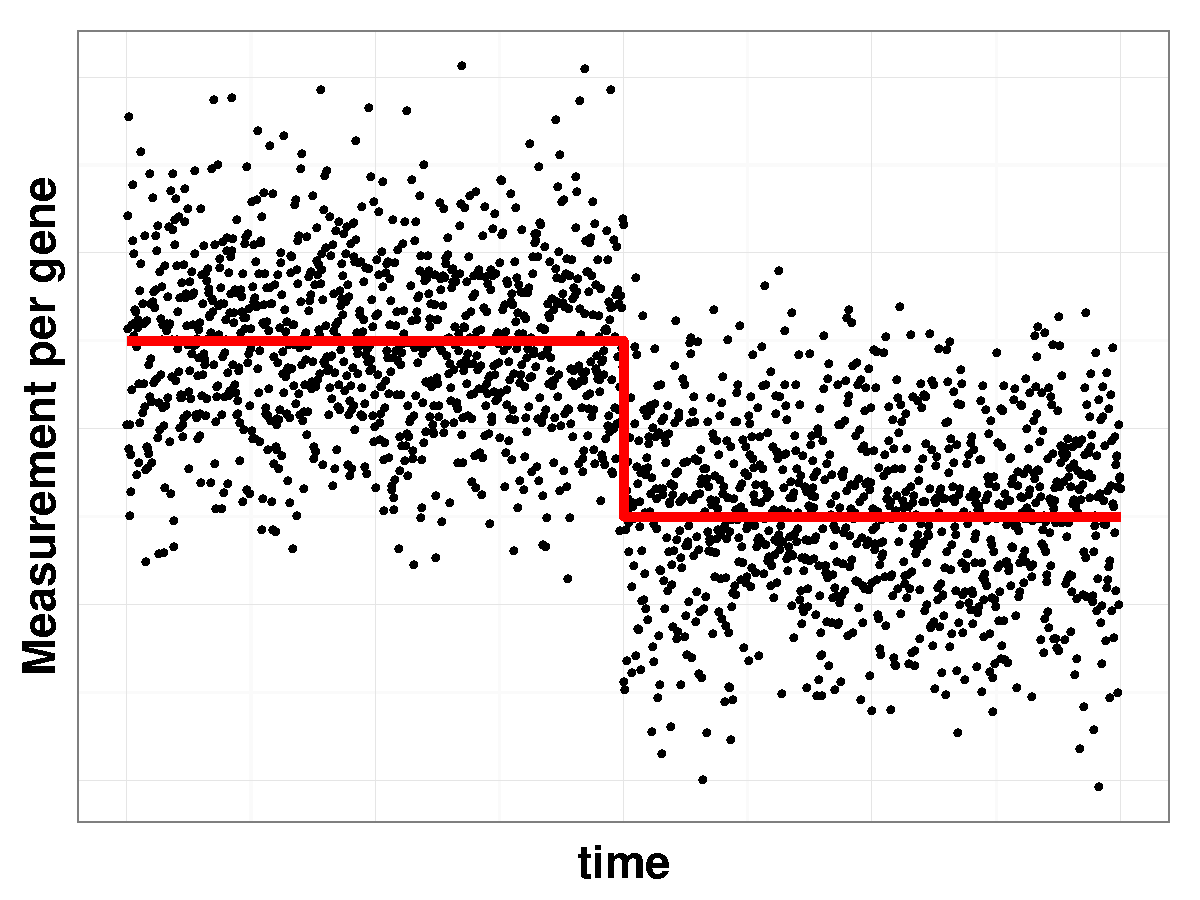
\includegraphics[width=0.45\textwidth]{pics/assmptn13.pdf} \label{fig:noninf-schem}
  }
  \subfigure[Gene not influential gradual change]{
    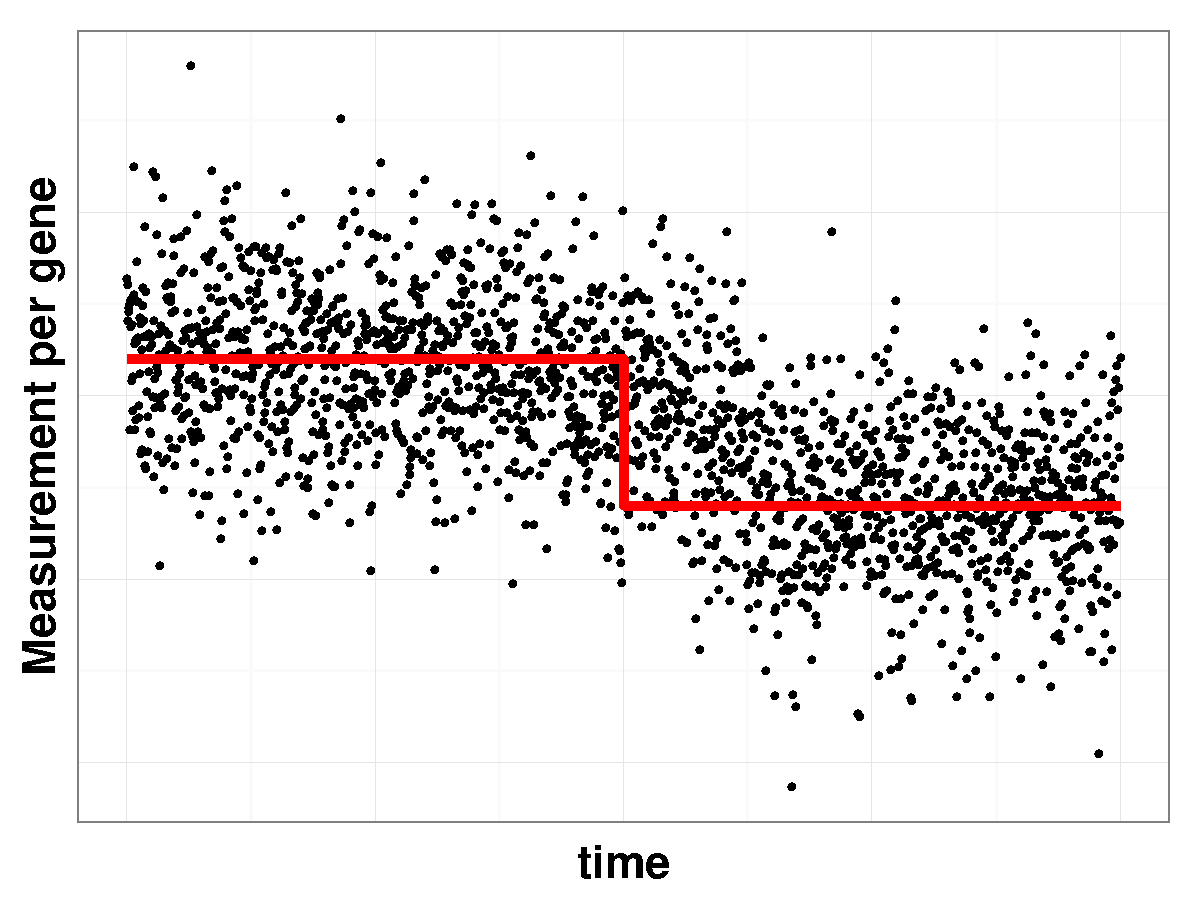
\includegraphics[width=0.45\textwidth]{pics/assmptn14.pdf} \label{fig:noninf1-schem}
  }
  \caption{
    Illustration. First assumption made is that gene expression remains constant for a gene while it remains inside a state. The model Section \ref{sec:markov-chain-master} describes the single cell measurement of a gene transitioning between states as an instantaneous step change (red line). In reality the measurement will at least fluctuate and transition won't be instantaneous. For influential genes \subref{fig:influential-schematic} - \subref{fig:influential1-schematic}, this assumptions is reasonable whether or not the transition is instantaneous, the points here are meant to represent single measurements. Genes where within state temporal changes are comparable to between state changes, \subref{fig:noninf-schem} - \subref{fig:noninf1-schem}, the approximation is not good. These genes are not influential for the transition process therefore this is not problematic.
 }
  \label{fig:schematic-ass1}
\end{figure}

A second assumptions relates to the topology of the Markov chain. To ensure parameter identifiability (see Discussion Section \ref{sec:identifiability}) we have to restrict the latent process to a linear pure birth process. This restricts the topology of the Markov chain quite drastically, but is arguably defensible when applied to externally driven transition processes. The external drive can take many different forms, in the two examples we investigate it is genetic induction. Of course back transitions are likely, for such cases our model is mis-specified and the forward transitions are only effective values where the back transitions have been absorbed into the model. Consequently estimated forward transitions rates are lower than the real values. On occasion back transitions or topologies of the latent process are of interest.
The likelihood eqn. (\ref{eq:likelihood}) is general and does not make any assumptions about the topology of the Markov chain, but additional data or constraints would be required for identifiability of more complex transition topologies. Often the limiting factor is available data hence we focus here on the more useful but special case where only time-course data is available and the latent stochastic process is a linear birth process. In Section \ref{sec:sim-study} we include a detailed investigation the impact of breaking this assumption in a simulation. 
% TODO refine ref to

Finally, we assume rates of cell death and cell duplication cancel each other out and the population therefore remains roughly constant in time. Consequently the fraction of cells in a given state only depends on the transition rates between the states. Especially in the case of oncogenic transformation (Section \ref{cha:oncog-transf}) this is clearly not the case since tumorous cells in general have a much higher proliferation rate. In Section \ref{sec:sim-study} we test how well parameters are estimated when this assumption is violated.

\subsection{Identifiability}
\label{sec:identifiability}

Parameter identifiability is a very important concept in STAMM since parameters represent physical properties of cells. A result for the identifiability of such a model with a discrete time latent process was present by \cite{Clifford:1977wa}. Unfortunately there do not exist a conclusive results on identifiability for latent stochastic model with a continuous time latent process. To establish if STAMM is identifiable analytically his highly non-trivial therefore we perform tests for empirical identifiability using single-cell simulations in Section \ref{sec:small-scale-model}. 

\section{Estimation}
\label{sec:estimation}

\subsection{Parameter estimation}
\label{sec:parameter-estimation}

We begin by stating the maximum likelihood estimates (MLEs) based on the likelihood eqn. (\ref{eq:likelihood}):

\begin{equation}
  \label{eq:leastSqrs}
  (\lbrace\hat{\beta}_j\rbrace, \hat{\mathbf{w}}) =  \underset{\lbrace\beta_j\rbrace, \mathbf{w}}{\operatorname{argmin}} \, \sum_{j=1}^p \sum_{t=1}^T \lVert g(x_j(t)) - g\left(P(t; \mathbf{w})\,\beta_j \right) \rVert_2^2,%+ \lambda \lVert \beta_j \rVert_1,
\end{equation}
where $\lVert \cdot \rVert_q$ denotes the $\ell_q$ norm with respect to its argument.
The transformation $g$ is in general non-linear as discussed above (e.g. $\log$ in microarrays or $\arcsinh$ in RNA-seq); for such transformations the MLE (\ref{eq:leastSqrs}) cannot be obtained in closed form. Genome wide measurements yield readings with number of genes, $p$, of up to $~10^4$. Directly optimising eqn. (\ref{eq:leastSqrs}) is not practical for a problem with large $p$ as the parameter space rapidly increases. We adopt a two-step estimation procedure proposed by \cite{Armond:2013}. The first step is based on the observation that many genes have similarities in their measured time-courses; this allows us to cluster genes obtaining $m$ clusters describing typical temporal patterns. Details for choosing the parameter $m$ are discussed in Section \ref{sec:estim-pipe}. The $m$ cluster centroids are used to estimate the transition rates $\mathbf{w}$ via eqn. (\ref{eq:leastSqrs}), instead of all genes. This approach reduces computation time significantly when $m << p$. 
The transition rates estimated using cluster centroids, $\hat{\mathbf{w}}$, are fixed and the $\beta$ values for all remaining genes are estimated. The MLE is now written as:
\begin{equation}
  \label{eq:leastSqrs.indep}
\hat{\beta}_j  =  \underset{\beta_j}{\operatorname{argmin}} \, \sum_{t=1}^T \lVert g(x_j(t)) - g\left(P(t; \hat{\mathbf{w}})\,\beta_j \right) \rVert_2^2 + \lambda \lVert \beta_j \rVert_1
\end{equation}
where the final term is an (optional) $\ell_1$ penalty with tuning parameter $\lambda$. It is invoked when potential over-fitting needs to be counteracted (choice of $\lambda$ is discussed in Section \ref{sec:estim-pipe}). 

The optimisation eqn. (\ref{eq:leastSqrs.indep}) greatly simplifies estimation (compared to  eqn. (\ref{eq:leastSqrs})), since estimation for individual $\beta_j$ for gene $j$ can be performed independently. This is possible because time-courses between individual genes are only coupled by transition rates $\mathbf{w}$; once they are fixed, individual gene trajectories can be examined independently. 

\subsection{Model selection}
\label{sec:model-selection}

The estimation steps described in Section \ref{sec:parameter-estimation} apply to a model with a fixed number of states $K$. Here we present a procedure to determine the number of states $K$ that best represent a data set under investigation. Depending on the application $K$ itself can be of scientific interest. In general estimated state-specific expression signatures, $\beta$, are influenced by the number of states. Underestimating number of states results in distinct states being merged. Overestimating the number of states introduces artificial states in the transformation. Both scenarios lead to poor estimation of parameters. 

In general model selection can be performed using a form of cross-validation (CV) by leaving out part of the data as a validation set. In some cases it is also possible to use BIC when the number e.g. when the number of genes is small, but this quickly breaks down as $p$ increases therefore we restrict ourselves to CV (see Section \ref{sec:model-selection-with} for further details). In applications to time-series, cross-validation is often non-trivial due to discrete and irregularly spaced observations. The STAMM model has an underlying continuous-time latent process, which allows for prediction of any time points from estimated parameters; therefore comparison between predicted time-points from estimated parameters and the corresponding held-out time-points. In this application due to poor time resolution it is often not possible to include more than one time point in the validation data; this variant is called leave-one-out cross-validation (LOOCV). If $t$ is the held-out time point let the estimated parameters for the remaining subset be rates $\hat{\bf{w}}^{-t}$, state specific expression $\lbrace \hat{\beta}_j^{-t} \rbrace$ and gene-specific standard deviation $\lbrace \hat{\sigma}_j^{-t} \rbrace$. State occupation probabilities at the held-out time point  $P(t; \hat{\bf{w}}^{(-t)})$ are obtained by solving the master equation using estimates derived from the training data. There we can now write a prediction for the expression of gene $j$ at the held-out time point $\hat{x}^{\mathrm{CV}}_j(t) = P(t; \hat{\bf{w}}^{(-t)})\, \hat{\beta}_j^{(-t)}$ and the cross-validation 
mean squared error ($\mathrm{MSE_{CV}}$) is simply
\begin{equation}
  \mathrm{MSE_{CV}}  =  \sum_{t=2}^T \sum_{j=1}^p \frac{1}{\hat{\sigma}_j^{(-t)}}\bigl( g(\hat{x}^{\mathrm{CV}}_j(t)) - g(x_j(t)) \bigr)^2.
  \label{eq:mse-cv}
\end{equation}

The strength of this type of model selection in comparison to the Bayesian approach presented in \cite{Armond:2013} is twofold. Firstly application of the computationally efficient estimation procedure outlined in Section \ref{sec:parameter-estimation}, allows this cross-validation procedure to be applied to the whole data set efficiently. Secondly it doesn't require parameters to be set by the user except those required for estimation. The Bayesian approach requires a computationally demanding Monte Carlo estimation and has several hyper-parameters which have to be set by the user. 

\begin{figure}
  \centering
  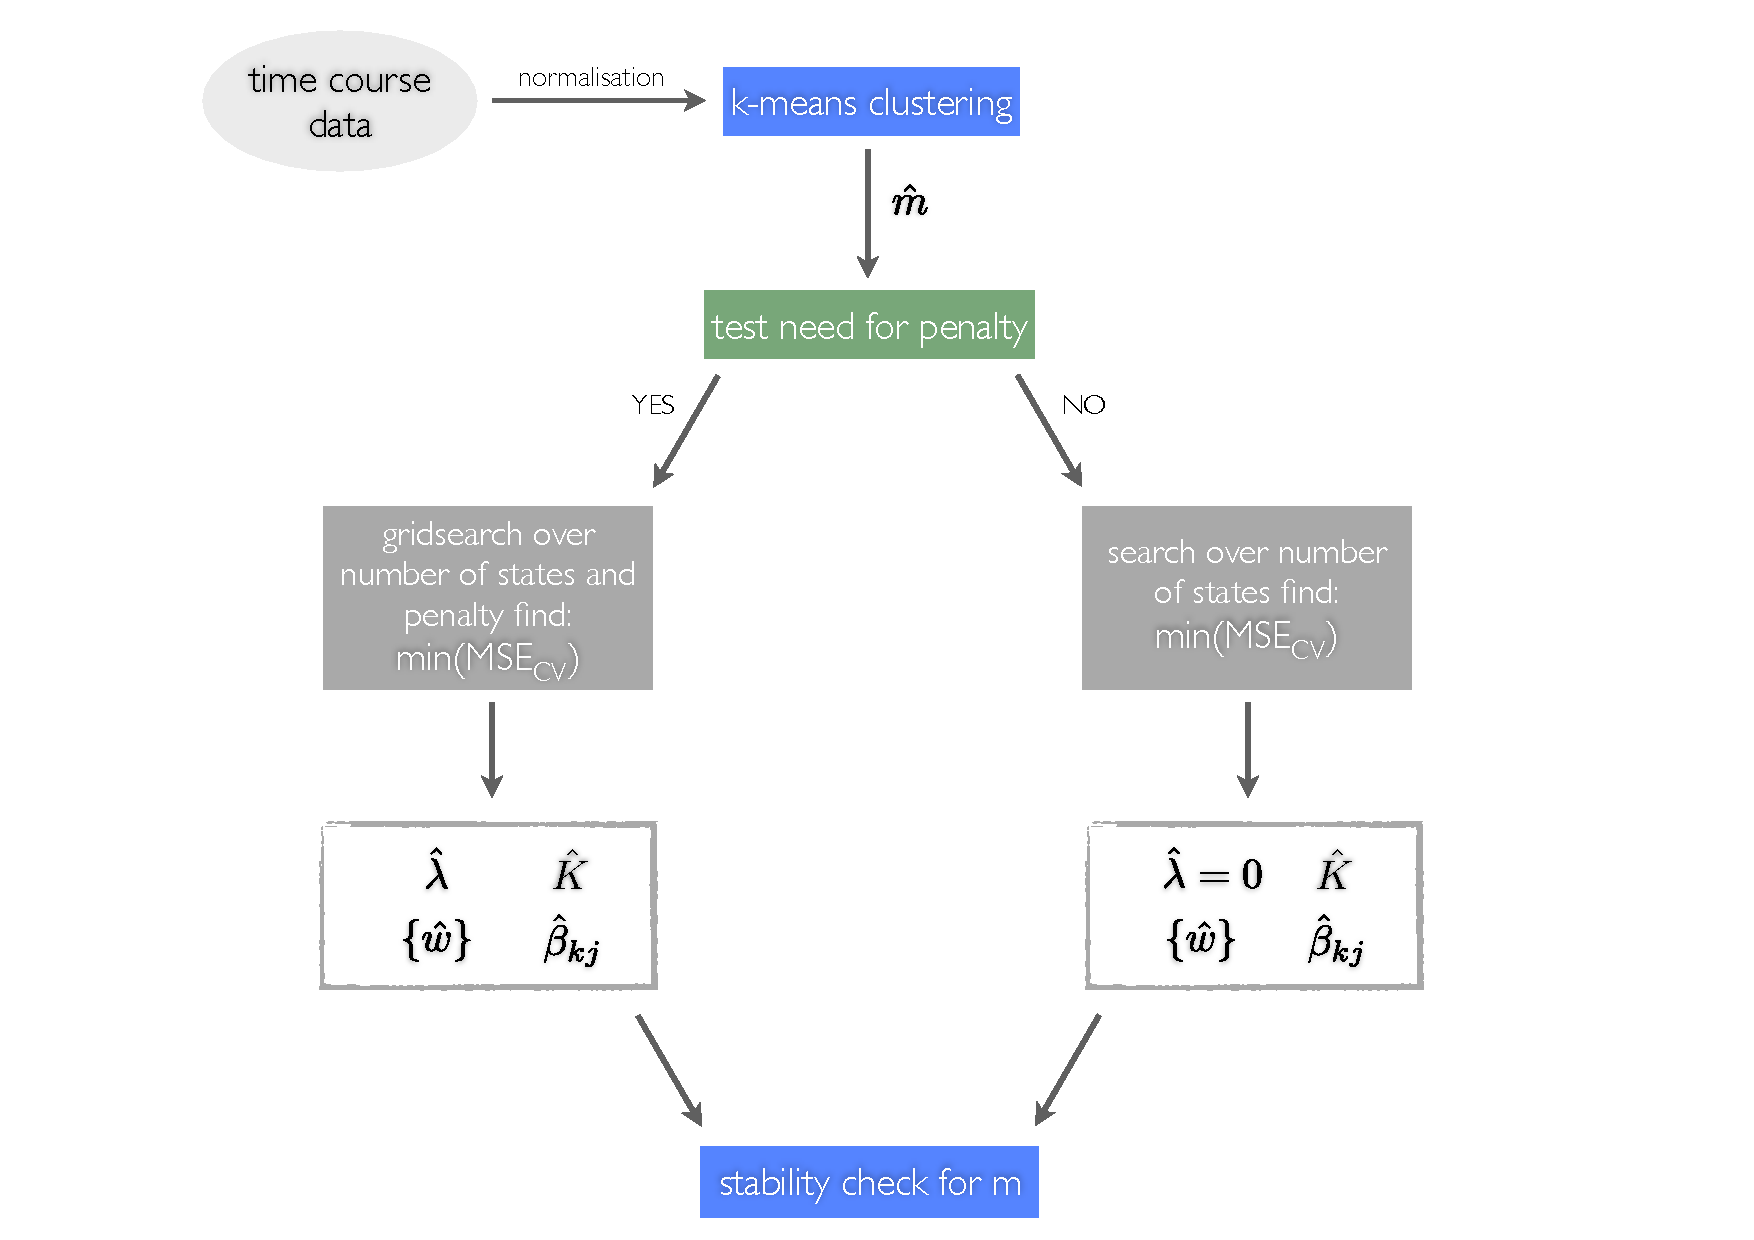
\includegraphics[width=0.9\textwidth]{pics/pipeline.pdf}
  \caption{Schematic of estimation pipeline. Clustering of normalised gene trajectories provides an optimum number of clusters $\hat{m}$, the centroids of the clusters summarise typical trajectories contained in data. Fitting the model to centroids we can find transition rates $w$. Stability of estimate test is performed to determine the need for penalisation of model parameters with strength $\lambda$. State-specific gene expression signatures $\beta_{kj}$ are estimated by varying the number of states in the model $K$ and $\lambda$ (if applicable). Optimum number of states are determined by performing a form of cross-validation. Finally sensitivity of estimation to change in $\hat{m}$ is performed. If necessary the pipeline is rerun with a better choice of $\hat{m}$.}
  \label{fig:pipeline}
\end{figure}

\subsection{Estimation pipeline}
\label{sec:estim-pipe}

We now present a computationally efficient pipeline for setting tuning parameters required for estimation. The pipeline is also summarised in Figure \ref{fig:pipeline}. The required tuning parameters are:

\begin{itemize}
\item The number of clusters, $m$, used in the first step of the two-step estimation.
\item The strength of the penalty term, $\lambda$, applied in eqn. (\ref{eq:leastSqrs.indep}), where $\lambda=0$ is equivalent to no penalty.
\item The number of states in the latent Markov chain, $K$.
\end{itemize}

\paragraph{Number of cluster:}
\label{sec:number-cluster}

In the initial estimation step we cluster gene expression trajectories which results in cluster centroids describing typical trajectories; these permit estimation of transition rates. In empirical results (see Section \ref{sec:large-scale-model}) we see; if the number of clusters is large enough to capture most of the information in typical trajectories changing $m$ does not have a significant impact on parameter estimation. Therefore we set $m$ using a simple k-means algorithm and inspecting the relative decrease of within-cluster sum of squares objective $J(m)$ as a function of $m$:

\[
\Delta J(m) = \frac{J(m-1) - J(m)}{J(m - 1)}
\]

We select $\hat{m}$  such that $\hat{m} = \min \lbrace m : \Delta J(m-1) < 0.1 \rbrace$, i.e. if the relative decrease in the objective function is smaller than $0.1$ for $m-1$ we choose $m$ as the number of clusters. Small fluctuations in the objective function for higher $m$ lead to instabilities in the relative decrease. Once $\hat{m}$ is set we include a post-estimation sensitivity test for the choice of $m$. In section \ref{sec:large-scale-model} we demonstrate with the help of empirical results, how well behaved and computationally efficient this model is. Though it should be noted that the choice of $m$ can be made with any clustering method and the corresponding objective function.

\paragraph{Penalisation:}
\label{sec:penalization}

The penalty term introduced in eqn. (\ref{eq:leastSqrs.indep}) is useful in high-dimensional models; even though the data investigated using this model will often be high dimensional, estimation is carried out separately for each gene. Therefore penalisation may not be required unless the number of time points is large. Consequently we introduce an additional step to test the need for penalisation by comparing estimated expression signatures $\beta$ with estimates obtained from leaving out individual time points. We specify stability as a Pearson correlation between estimated $\beta$ values  greater than $0.8$. If we deem a data set stable under such a test there is no need for penalisation and we choose $\lambda=0$. If the correlation is smaller than $0.8$ a penalty term is required (setting the penalty strength is discussed below). In both the simulated data sets and application to oncogenic transformation penalisation was not required and $\lambda=0$ in Sections \ref{sec:results} and \ref{cha:oncog-transf}. 

\paragraph{Number of states:}
\label{sec:number-states}

The final parameter to be set is the number of states in the latent Markov chain. This parameter is set by minimising the CV score ($\mathrm{MSE_{CV}}$) for a range of different $K$. If penalisation is required $\mathrm{MSE_{CV}}$ is minimised by performing a grid search over both $\lambda$ and $K$.

All three parameters ($m$, $\lambda$, $K$) can in principle be set by performing a grid search with respect to $\mathrm{MSE_{CV}}$, but this is computationally very challenging and would make estimation impractical. Our pipeline make use of heuristic observations to reduce the grid search to one dimension. The observation that estimates are robust to the choice of the number of clusters allows us to remove $m$ from the grid search. Observing that the penalty term is not always needed enables us to exclude $\lambda$ from the grid search. When choosing $m$ using a clustering method it could be that transition rates haven't converged. Therefore we carry out an additional diagnostic post estimation. The issue we are trying to address is that an increase in $m$ corresponds to an increase in information; this can lead to changes in estimated parameters. If the choice is appropriate parameters estimated increasing the number of clusters should not significantly impact parameters. To this end we compute correlation values between expression levels $\beta$ estimated using $\hat{m}$ clusters and estimated using larger values $m' > \hat{m}$. Provided results have Pearson correlation above $0.8$, the choice of $\hat{m}$ was appropriate, if the correlation is below $0.8$ we repeat the pipeline with larger $m$. 

\section{Simulation setup}
\label{sec:sim-study}

To test the validity of the model we need to test it with simulated data where true parameters are known. This will allow both evaluation of strengths and weaknesses in parameter estimation and model selection (choosing number of states). Simulations are performed not at the cell population level of the likelihood eqn. (\ref{eq:likelihood}) but at the single-cell level; allowing for extensive testing of model assumptions. The single cell trajectories are then averaged to obtain homogeneity data analogous to RNA-seq data.

Here we describe the step by step simulation procedure for a $K$ state model independent of the number of genes simulated:

\begin{figure}
  \centering
  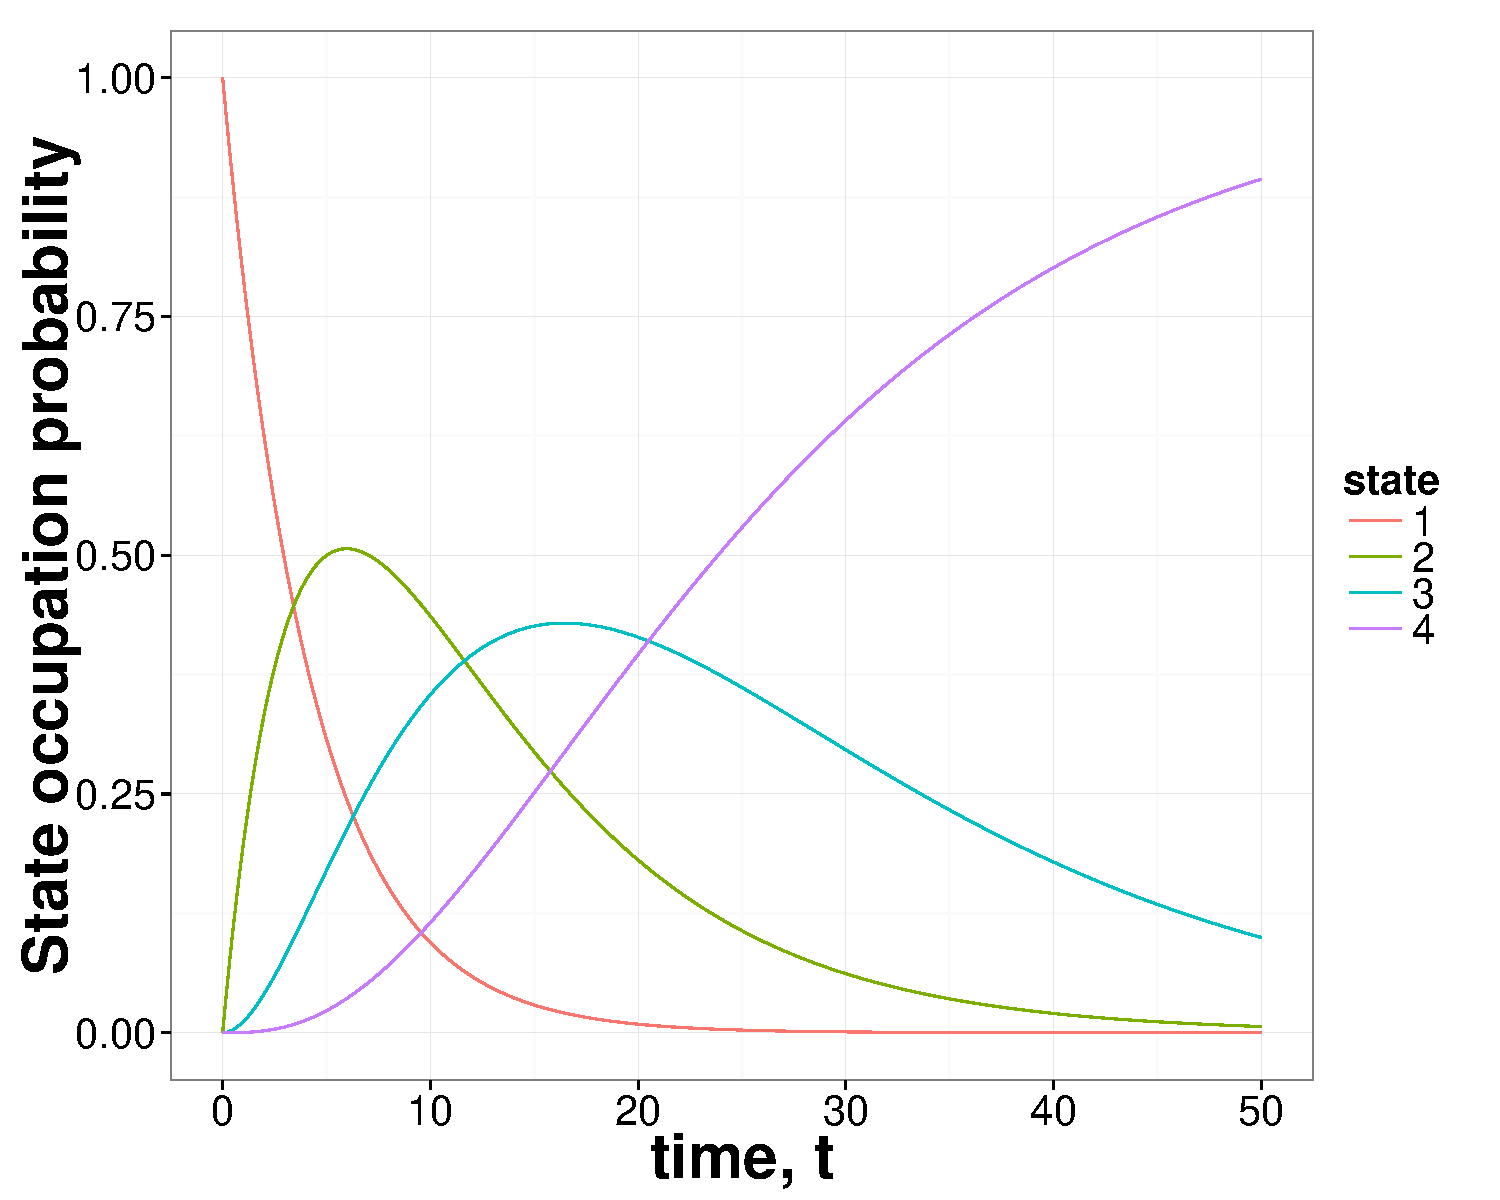
\includegraphics[width=0.7\textwidth]{pics/trans-rates.pdf}
  \caption{Simulation study. State occupation probabilities for a four state model with transition rates $[1/5, 1/8, 1/15]$. The transition rates are set to these values for all simulations, the values are chosen to allow $k=4$ to have a high occupation probability at the final time-point of the simulation.}
  \label{fig:transition-rates}
\end{figure}

\paragraph{State transitions.}
\label{sec:state-transitions}

When setting transition rates between discrete states of the Markov chain we need to keep a few things in mind. Firstly the smallest sampled (observed in real data) time step needs to be smaller than the transition rates. Just like in typical experimental designs for transition processes. Additionally the model won't be able to extract information about a process taking place on a time-scale smaller than gaps between observations. Secondly we are considering transitions processes driven towards an established final state (e.g. oncogenic transformation, pluripotency); so to mimic this behaviour in simulated data we need to insure the occupation probability for the final state is higher than the others at the final time point. Of course in realistic experiments even at the final time point the cell population will still be heterogeneous In the discussion that follows in Section \ref{sec:results} we use the three transition rates $[1/5, 1/8, 1/15]$ for four state model. In Figure \ref{fig:transition-rates} we show the state occupation probabilities for these parameters and $k=4$ has an occupation probability of $\approx 0.89$ at the final time point. For every cell in the simulation, state transitions are simulated by drawing jump-times from exponential distribution with parameters given by transition rates as defined for a continuous-time Markov chain.

\paragraph{State-specific expression levels.}
\label{sec:state-spec-expr}
For all cells, each gene $j$ and state $k$ we set gene expression levels $\beta_{kj}$; per gene the expression levels are set to zero with probability $1/K$ otherwise they are sampled uniformly from $(0, \gamma_j]$. Parameter $\gamma_j$, chosen from the range $[1, \ldots, 12000]$, effectively sets the scale of gene $j$ \footnote{It is always chosen from the following $\gamma_j = \lbrace 1, 10, 50, 100, 200, 500, 1000, 2000, 4000, 7000, 10000, 12000 \rbrace$}. This method ensures simulated trajectories for genes on different scales (see Figure \ref{fig:small-sim-traj} and the corresponding gene expression signatures Figure \ref{fig:small-sim-beta}), to emulate real RNA-seq data  where a range of five order of magnitude was observed \citep{Wang:2009ur,Mortazavi:2008jj}. Gene expression trajectories for single cells are piecewise flat for each gene once $\beta$ values are sampled. Changes in trajectories only occur at jumps between states and are instantaneous.

\paragraph{Aggregation and time-sampling.}
\label{sec:aggr-time-sampl}
For each gene $j$ each cell has an associated gene expression trajectory. Similar to RNA-seq experiments where observations are averages of gene expressions over many cells; these trajectories are averaged over a large number of cells to give an average gene expression trajectory. The occupation probability in the model outlined in Section \ref{sec:mast-model} is derived in the limit of number of cells $\rightarrow \infty$, of course in practice the number of cells is finite. We set the number of cells to $1000$ which serves as a good test of the limiting assumption.

The simulated time-course is obtained by sampling the simulated trajectories at discrete unevenly distributed time points. Finally Gaussian noise is added to the transformed data (see Section \ref{sec:mast-model} for details, for RNA-seq $\arcsinh$) with mean zero and standard deviation $\sigma$; which we set to $\sigma=0.2$ unless states otherwise, this provides a reasonable signal to noise ratio for all observations. Similar to the RNA-seq data discussed in Section \ref{cha:oncog-transf} we choose $15$ unevenly spaced  time points at $t=\lbrace 0,  2,  4,  7,  8, 11, 14, 20, 24, 29, 32, 35, 40, 44, 48\rbrace$. The simulation setup is summarised in pseudocode in Algorithm \ref{alg:simulation-framework}. 


\begin{algorithm}
    \caption{Pseudocode for single cell simulations}\label{alg:simulation-framework}
    \begin{algorithmic}[0]
        \Procedure{Simulation}{$n.states, n.genes, n.cells, r, p, \tau, dt$}
        \State $\beta \gets   NB(r;p)$
        \State $jump.t \gets Exp(1/\tau_k)$
        \ForAll{$genes, cells$}
        \For{$t  \gets 0,T$}
        \While{$t < jump.t_{states}$}
        \State $sim.traject(t) \gets \beta_{j,k}$
        \EndWhile
        \EndFor
        \EndFor
        \State average $sim.traject$ per gene for all cells
        \State $sim.data \gets sim.traject$ (sampled at discrete time)
        \State $sim.data \gets sim.data$ + $\mathcal{N}(0, \sigma)$
        \EndProcedure
      \end{algorithmic}
\end{algorithm}

\section{Simulation results}
\label{sec:results}

We present results from simulations in two separate phases. For both simulation setup the transition rates are fixed at $[1/5, 1/8, 1/15]$ and we simulate from a model with four states in latent Markov chain. First in a small scale simulation with $p=9$ genes we perform multiple rounds of direct estimation of the whole data without the need for the initial clustering step. This simpler simulations allows investigation of identifiability and an investigation for model selection without considering the two-step estimation procedure outlined above.

Than we consider a larger scale simulation with $p=120$ genes, where we put the full two-step estimation procedure to the test; including clustering, setting of tuning parameters and finally model selection.



\subsection{Small scale simulation}
\label{sec:small-scale-model}

Using the small scale simulation we perform three separate  tests. One in which we only estimate transition rates and state-specific expression levels; we consider the number of states to be known. Then we consider the model selection problem and finally we investigate estimation under breaking model assumptions.

\subsubsection{Number of states known}
\label{sec:number-states-known}

We simulated $9$ genes from a $4$ state model as described in Section \ref{sec:sim-study}. In this small simulation we do not use a penalisation term, i.e. $\lambda=0$. In Figure \ref{fig:small-sim-traj} we show trajectories for one such realisation, here the thicker line represents trajectories from averaging $1000$ cells for each gene. The green dots show sampled data with the addition of Gaussian noise to transformed data. In Figure \ref{fig:small-sim-beta} we show state-specific gene expression signatures for all $9$ simulations. The values are shown in pairs of true and estimated. The value on the right is in each case the true value used in simulating the trajectories. The left-hand value is estimated by fitting the $15$ time point of the simulation. The corresponding estimated and true transition rates for this realisation can be seen in Table \ref{tab:fit-w}. Using the estimated transition rates and the expression signatures we can obtain an estimated trajectory, seen as a blue line in Figure \ref{fig:small-sim-traj}.

\begin{figure}
  \centering
  \subfigure[Simulated Trajectories for $p=9$] {
    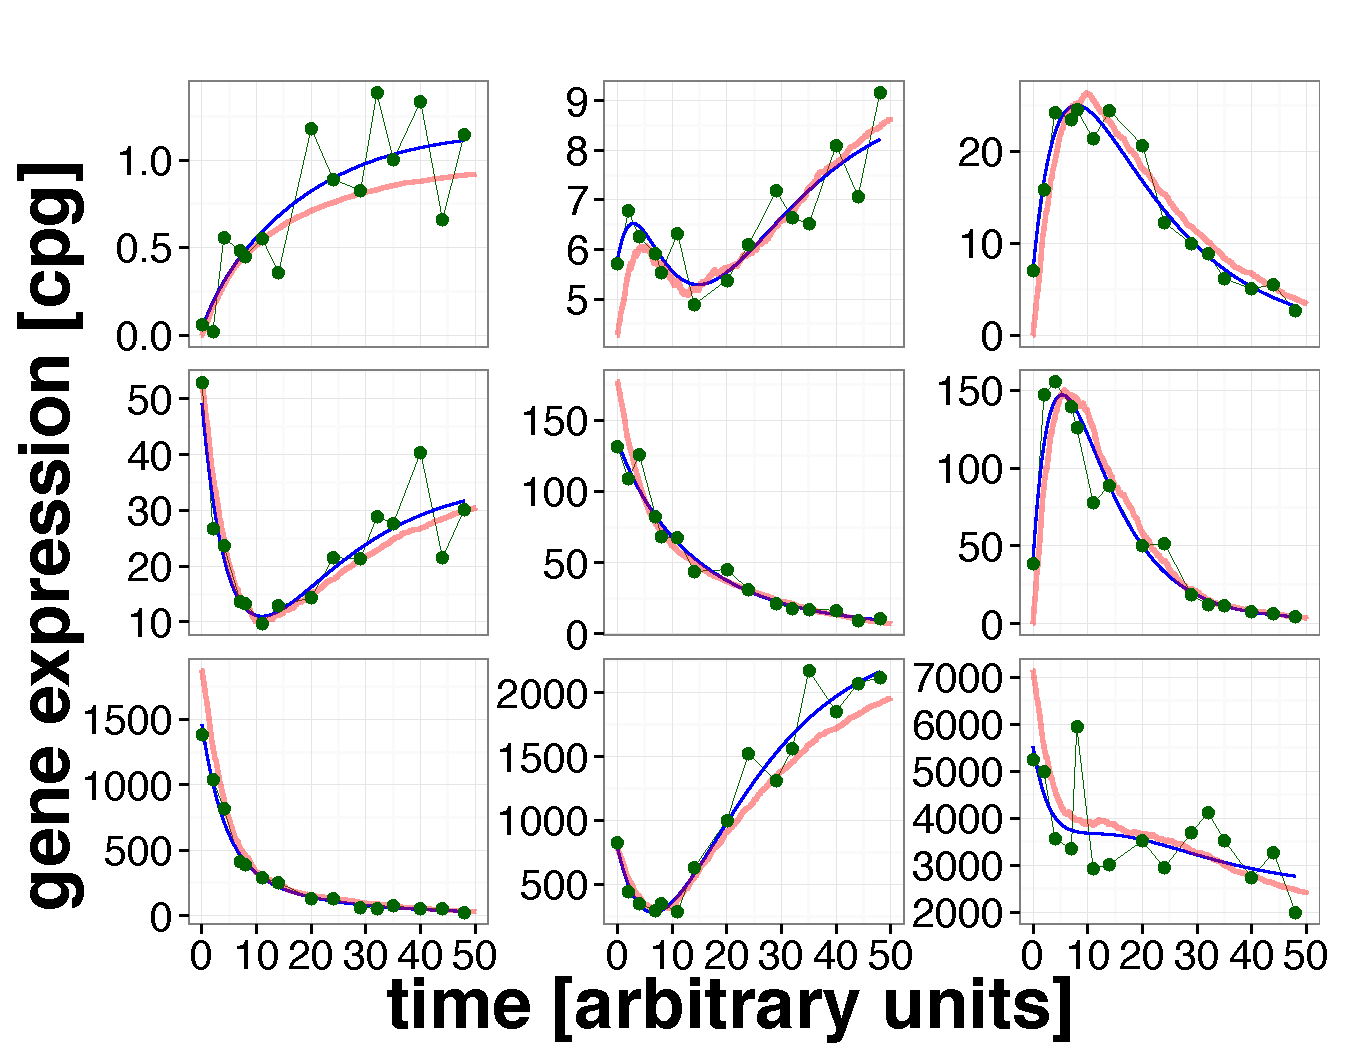
\includegraphics[width=0.6\textwidth]{pics/traj-comp.pdf}
    \label{fig:small-sim-traj}
  }
  \subfigure[Expression signatures for $p=9$ simulation] {
    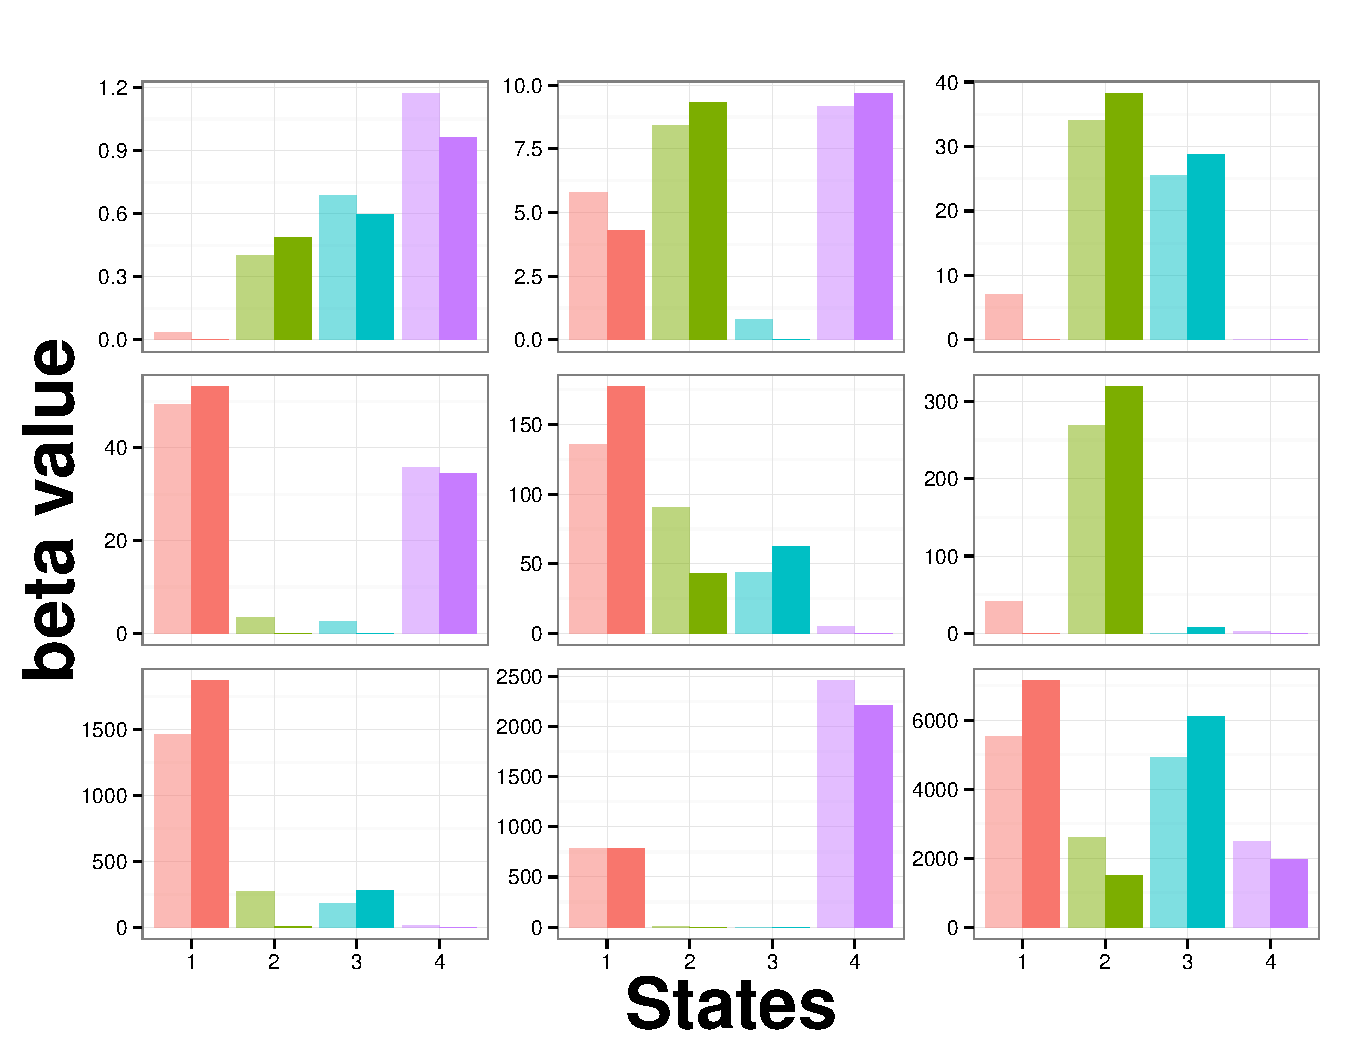
\includegraphics[width=0.6\textwidth]{pics/beta-comp.pdf}
    \label{fig:small-sim-beta}
  }
  \caption{Simulation study. Small scale simulation for $p=9$ genes. \subref{fig:small-sim-traj} shows the trajectories for these simulations. The thick red line shows the averaged trajectories over $1000$ cells. The green dots show $15$ sampled data points with normal noise ($\mathcal{N}(0, \sigma)$, with $\sigma=0.2$) added to the average data. The blue thin line shows the trajectory from estimated parameters. \subref{fig:small-sim-beta} shows state-specific gene expression signatures for all $9$ simulated genes. The true and estimated parameter values are shown next to each other. The lighter colour on the left shows estimated parameter values, the solid colours shows true parameter values.} 
  \label{fig:small-scale-sim}
\end{figure}

\begin{table}[h]
    \centering
\begin{tabular}{r|rrr}
  \hline \hline
  \bf{Transition rates}& $w_{1,2}$ & $w_{2,3}$ & $w_{3,4}$ \\ 
  \hline
  true mean & 0.200 & 0.125 & 0.067 \\ 
  estimated & 0.236 & 0.114 & 0.068 \\ 
   \hline
 \end{tabular}
 \caption{Transition rates used in the simulation and the estimated values}
 \label{tab:fit-w}
\end{table}

We repeat fifty such independent simulations at four different noise levels \footnote{$\sigma=\lbrace 0.05, 0.1, 0.15, 0.2 \rbrace$d}, each time $\beta_{kj}$ are resampled as described above (Section \ref{sec:state-spec-expr}) while transition rates are shared across simulations. We compute the correlation between estimated and true gene expression signatures for each simulation run $\rho(\beta,\hat{\beta})$. The correlation coefficients for all simulations are summarised in a boxplot, Figure \ref{fig:sim-fifty-beta}. For all tested noise levels we compute a mean and standard deviation of the correlation coefficient across all fifty runs in Table \ref{tab:cor-beta-fifty}; The mean is above $0.9$ for all simulations and the highest level for the variance is $0.13$. Therefore we can conclude that that state-specific gene expression signatures are recovered well in the simulation. We also introduce a new measure, $s_k = \lvert \hat{w}_{k,k+1} - w_{k,k+1} \rvert$ to test recovery of transition rates. For each simulation we use the mean $\bar{s}$ over the three transition rates as measure for how well transition rates are recovered. In Figure \ref{fig:sim-fifty-w} we show boxplots for the fifty simulations for each of the four noise levels. We find that transition rates are also recovered well, though as expected the estimates become worse with increasing noise levels.

\begin{table}[ht]
\centering
\begin{tabular}{rrrrr}
  \hline
$\sigma$ & 0.05 & 0.1 & 0.15 & 0.2 \\ 
  \hline
mean & 0.95 & 0.93 & 0.94 & 0.91 \\ 
std. dev. & 0.07 & 0.09 & 0.08 & 0.13 \\ 
   \hline
 \end{tabular}
 \caption{Correlation between true and estimated gene expression signatures. Mean and standard deviation are estimated across $50$ independent simulations.}
 \label{tab:cor-beta-fifty}
\end{table}

\begin{figure}
  \centering
  \subfigure[State-specific gene expression]{
    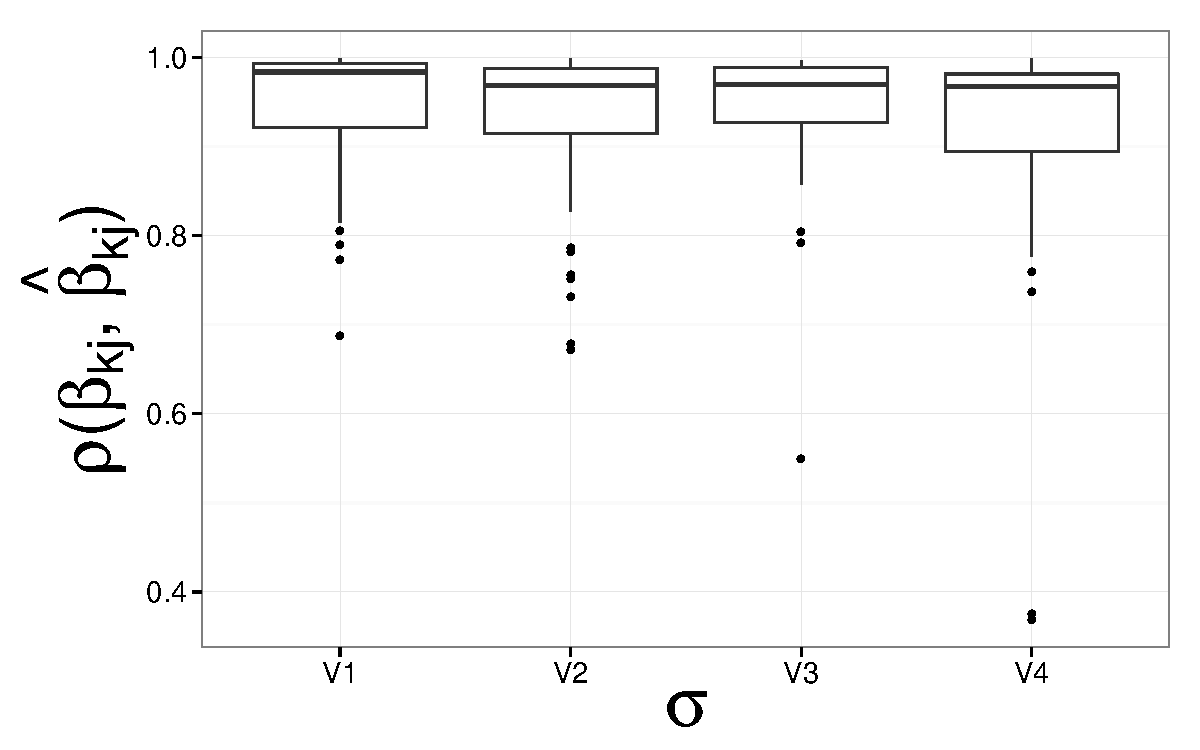
\includegraphics[width=0.47\textwidth]{pics/correlation.pdf}
    \label{fig:sim-fifty-beta}
  }
  \subfigure[Transition rates]{
    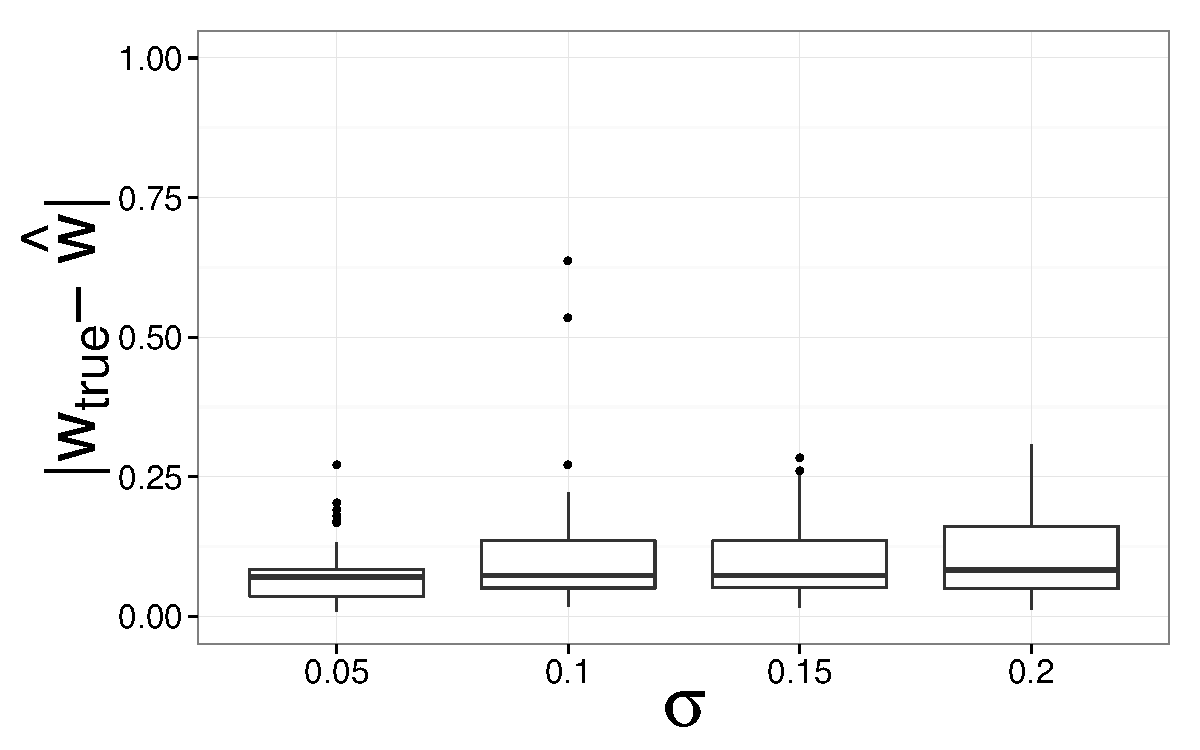
\includegraphics[width=0.47\textwidth]{pics/mean-diff.pdf}
    \label{fig:sim-fifty-w}
  }
  \caption{Simulation study. Small scale simulation using $p=9$ genes with $50$ independent repeats. Boxplots show results over all repeated simulations at four different noise level $\sigma = \lbrace 0.05, 0.1, 0.15, 0.2 \rbrace $. \subref{fig:sim-fifty-beta} Boxplots for correlations between estimated and true gene expression signatures ($\rho(\beta_{\mathrm{true}},\hat{\beta})$) at four different noise levels. \subref{fig:sim-fifty-w} Boxplots for the mean of absolute differences between the estimated and true transition rates $\bar{s}$ for each simulation at four different noise levels. }
  \label{fig:small-scale-50}
\end{figure}

\subsubsection{Determine number of states}
\label{sec:determ-numb-stat}

Next we consider the problem of model selection in this small simulation setup. We simulate data as described above for $p=9$ genes. In such a model with a latent stochastic process, model selection is a challenging problem especially using noisy data sets. Therefore to test model selection we fifty independent simulations for each of the following noise regimes: $\sigma = \lbrace 0.05, 0.1, 0.15, 0.2 \rbrace $. We compare models with $K = 1 \ldots 5$ and perform model selection using leave-one-out cross-validation (see Section \ref{sec:model-selection}), for each of the fifty simulations. We determine the minimal $\mathrm{MSE_{CV}}$ scores (eqn. (\ref{eq:mse-cv})) for different models and juxtapose a comparison between the different models using a simple normalised MSE score for model fit without held-out time points. In each simulation and for each noise regime we determine the model with lowest $\mathrm{MSE_{CV}}$ score and lowest MSE score. Then we show the distribution of these minimal scores over the selected number of states in Figure \ref{fig:small-scale-modelSlct}; the top row shows the distribution for $\mathrm{MSE_{CV}}$ and bottom row show the distribution for MSE in different noise regimes. 

Here number of parameters increase with number of states, and as a result model fit improves; therefore as expected at all noise levels the maximum number of states ($K=5$) results in the best fit. 

\begin{figure}
  \centering
  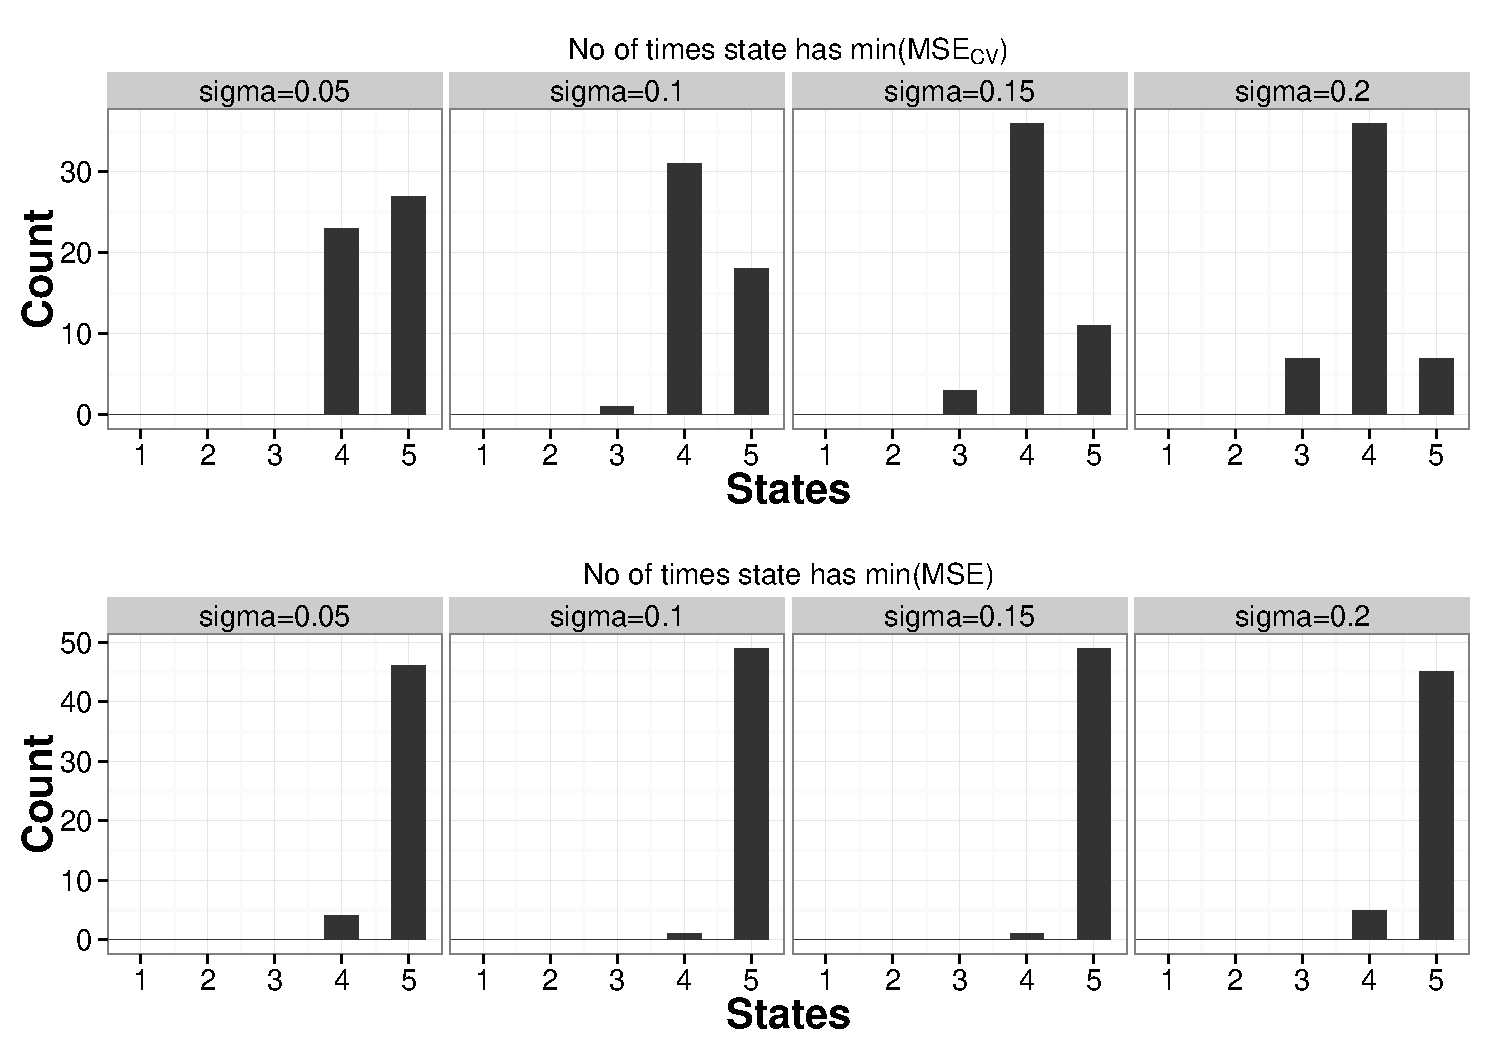
\includegraphics[width=0.9\textwidth]{pics/hist-all.pdf}
  \caption{Simulation study. We perform fifty independent small scale simulation with $p=9$ at four different noise levels $\sigma = \lbrace 0.05, 0.1, 0.15, 0.2\rbrace$ for $K=4$. We perform model selection using a form of cross-validation and find the state $K$ that minimises the $MSE_{CV}$ score, top row. As a comparison we also show fit to data and find the state $K$ that minimises $MSE$. We find that at even at very high noise levels using $MSE_{CV}$ it is possible to identify the right model. An example trajectory and parameters can be seen in Figure \ref{fig:small-scale-sim}.}
  \label{fig:small-scale-modelSlct}
\end{figure}

\subsubsection{Violating model assumptions}
\label{sec:viol-model-assumpt}

Until now we have considered simulations with a correctly specified model where assumptions underlying the model are not violated. Breaking these assumptions is especially easy in the single cell simulation. We investigate consequences on parameter estimation under violation of a subset of these assumptions. We use three types of plots to investigate parameter estimation for these simulations. 

\begin{itemize}
\item {\bf Correlation.} For state specific gene expression signatures $\beta_{kj}$ we compute the Pearson correlation coefficient between true parameters and estimated parameters, $\rho(\beta_{\mathrm{true}},\hat{\beta})$.
\item {\bf Transition times.} We show boxplots of estimated average transition times for $10$ simulations and a horizontal dashed line to represent the true value used in the forward simulation.
\item {\bf Probability} In the model itself the transition times do not enter directly they are used to calculate probabilities. We compare the values by calculating a mean difference between probabilities:
\begin{equation}
  \label{eq:1}
  \left< \lvert \hat{p}_k(t) - p_k(t) \rvert \right>_{k,t}, 
\end{equation}
where $k$ is the number of states, $\hat{p}_k(t)$ is the probability calculated from estimated parameters and $p_k(t)$ is
the probability calculated from true values. The average is taken over both the states and time. 
\end{itemize}



\subsubsection{Cell death and cell doubling}
\label{sec:death-duplication}

\begin{figure}
  \centering
  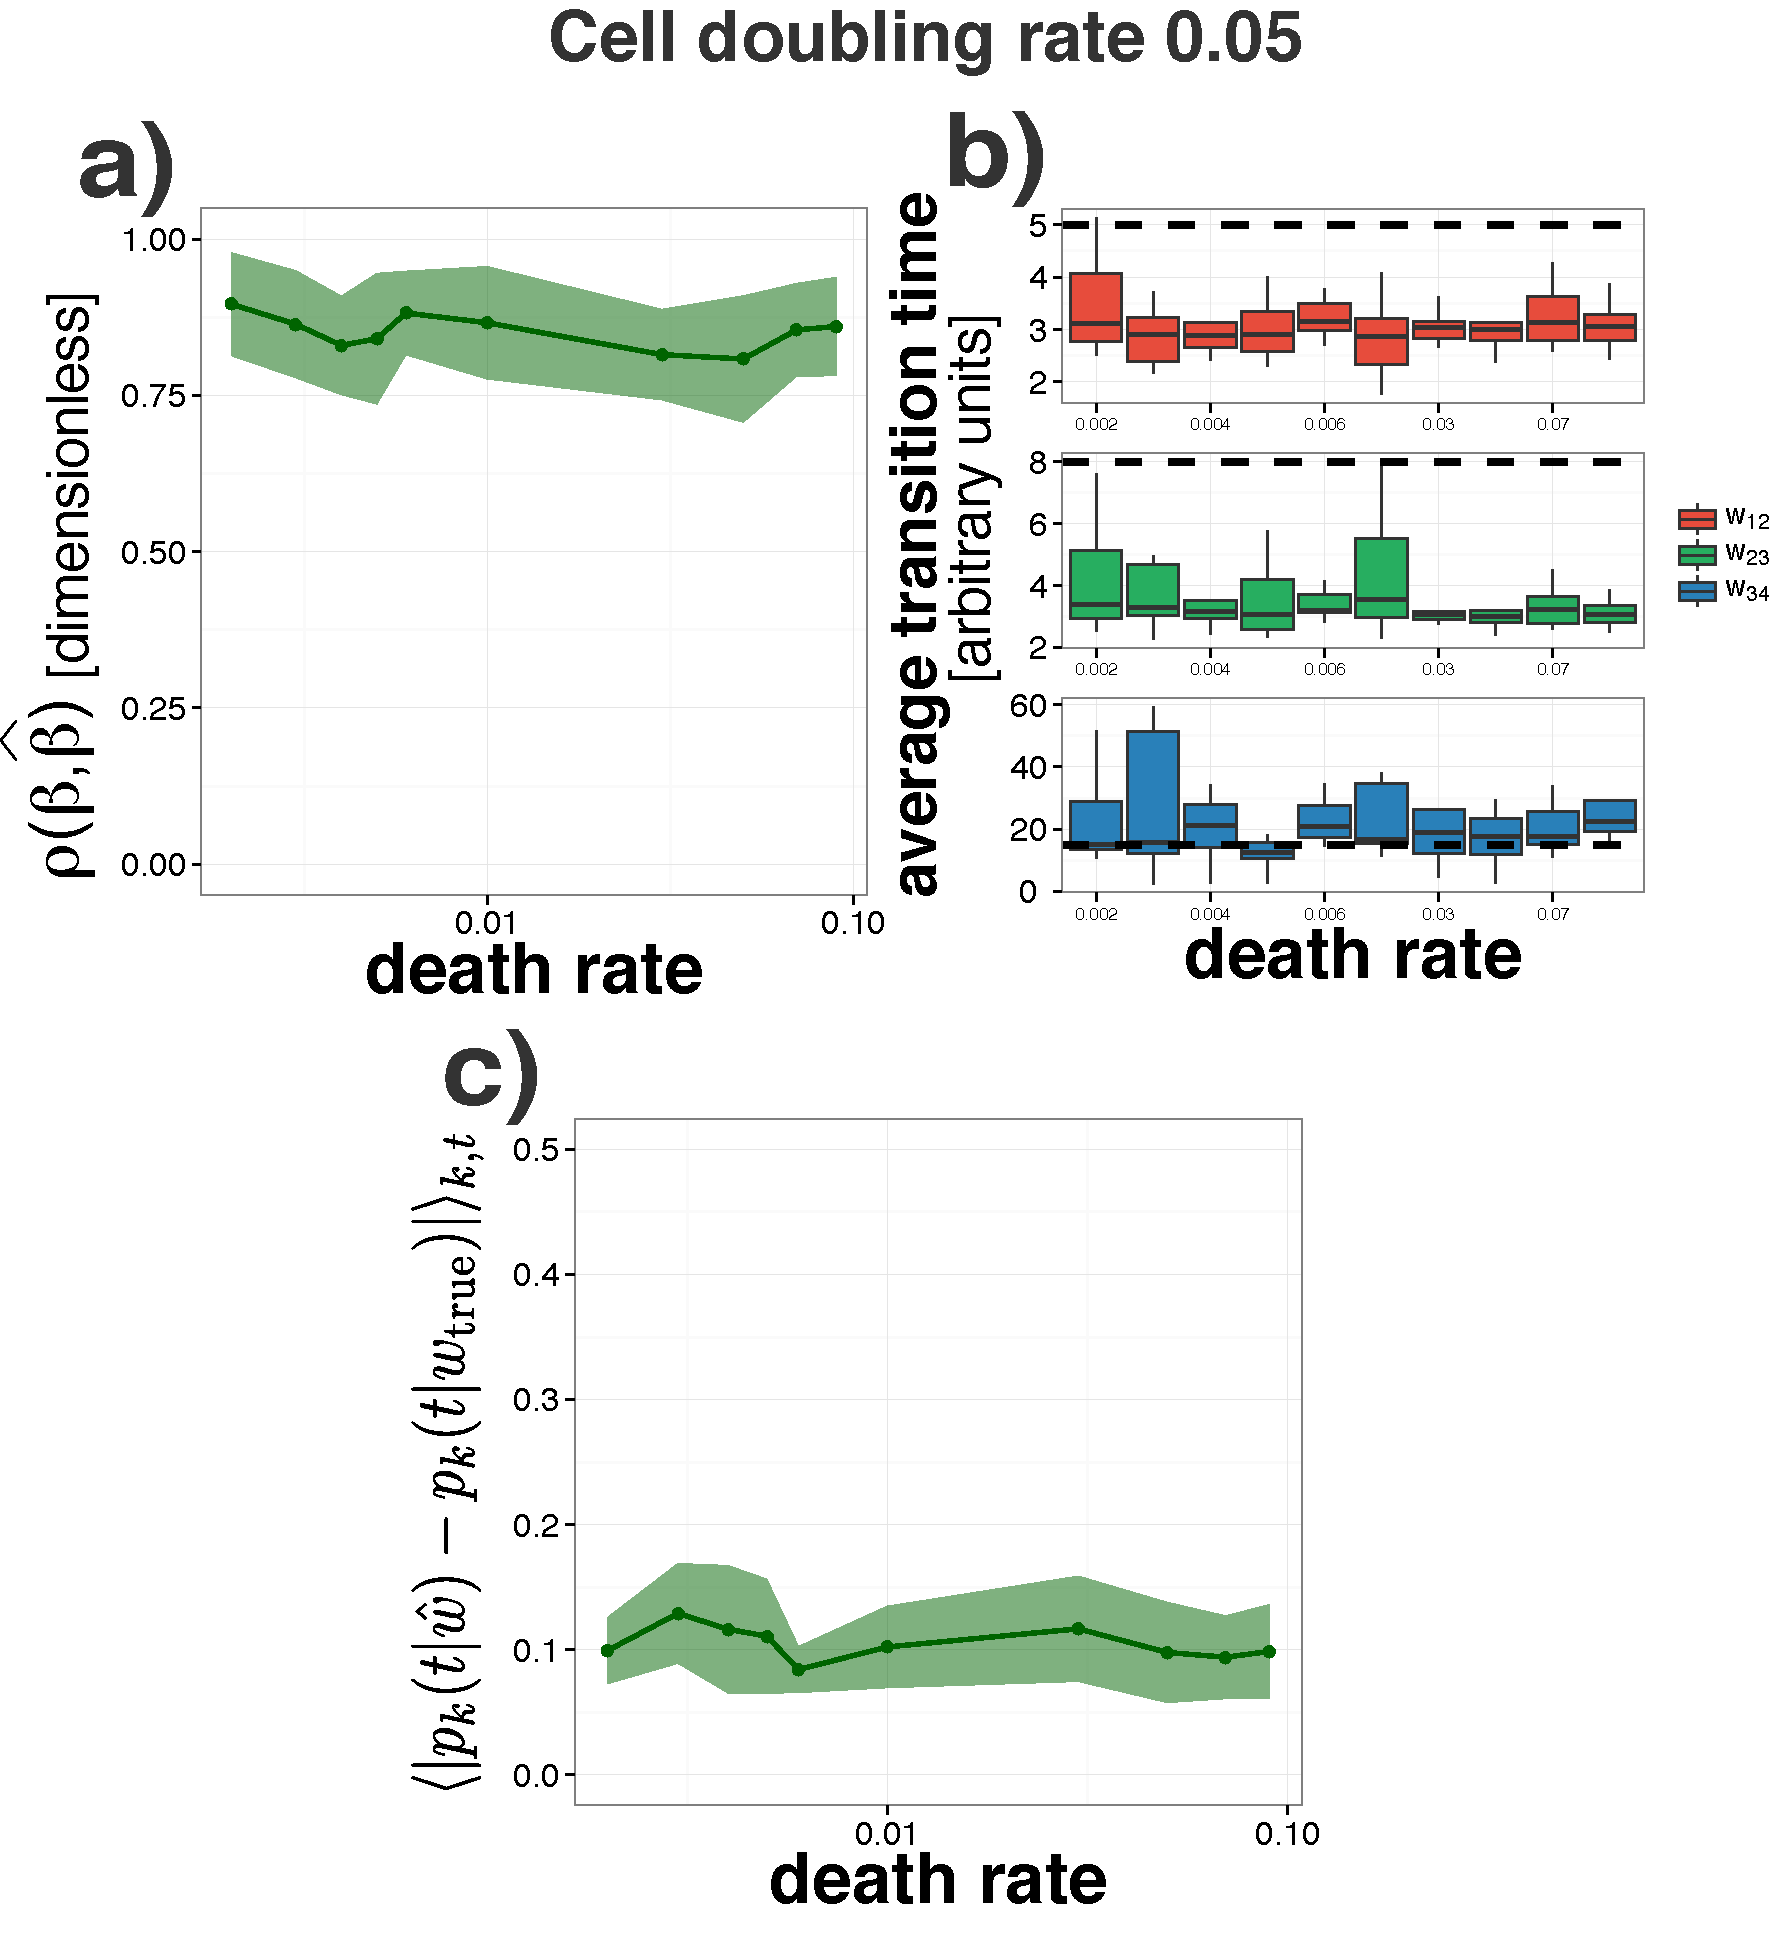
\includegraphics[width=0.9\textwidth]{pics/realist-dupl.pdf}
  \caption{Simulation study. Testing assumption about cell death and cell doubling. For each cell a time of death, $t_i^{d}$, and a time for cell doubling, $t_i^{dup}$, is sampled from an exponential distribution with varying average rates. If the sampled rates for a cell are outside of the time range of the simulation, the cell remains unchanged. If they are both in the range there are two options. The first option is that the death rate is the smaller of the two in that case the cell $i$ is taken out of the simulation $t>t_i^d$. If $t_i^{dup}<t_i^d$, cell $i$ is taken out of the simulation at $t > t_i^{dup}$ and two new cells are simulated with new state transitions. The simulation and fit is performed $10$ times. In experiments we observe cell doubling time to be roughly 18 hours and very few dead cells. Therefore we simulation with a cell doubling rate of $0.05$ and a variety of death rates. The left panel shows the average as a dark line and the shaded area represents the standard deviation for the $10$ repeated simulations. The middle panel shows boxplots for the estimated average transition times. The right panel shows the mean differences between estimated and true probabilities averaged over $10$ trajectories as a solid line and the shaded area represents the standard deviation.}
  \label{fig:dupl-realistic}
\end{figure}

\begin{figure}
    \centering 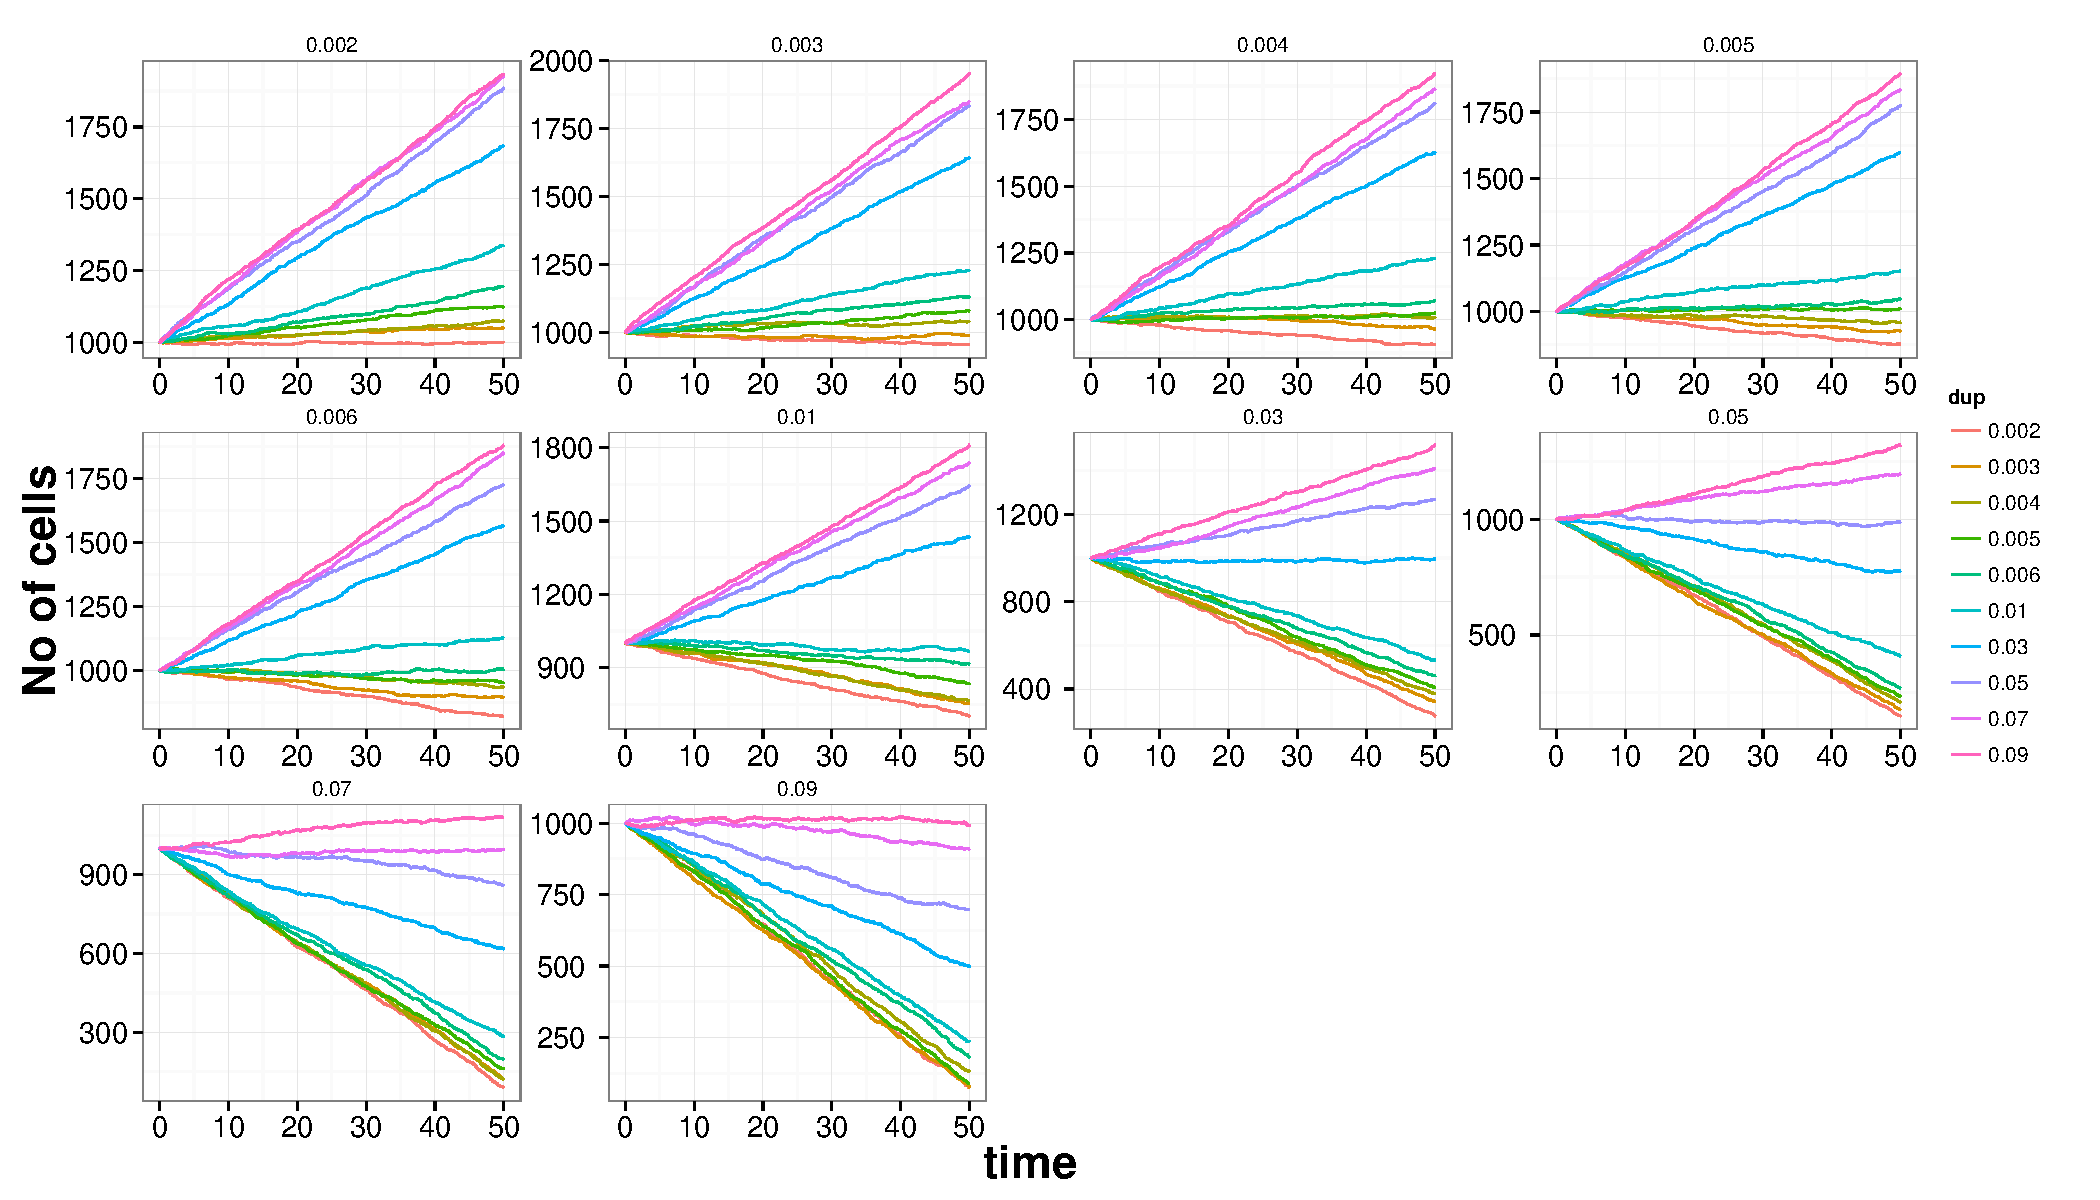
\includegraphics[width=1\textwidth]{pics/n-cell.pdf}
    \caption{Simulation study. Testing assumptions about cell death and cell doubling. Plots show number of cells at different time during the simulation for one of the $10$ simulations. Each panel represents different death rates and each colour different doubling rates.}
\label{fig:no-cells-dupl}
\end{figure}

An assumption implicit in STAMM is that cell death and cell duplication happens at a constant rate across all states in the transformation process. This is of course not the case in the discussed example of oncogenic transformation, since transformed tumorous cells have a much higher proliferation rate than the initially healthy cells. In the single cell simulation setup we sample a time of death, $t_i^{d}$, and a time for cell doubling, $t_i^{dup}$, from an exponential distribution. If sampled rates for a cell are outside of the time range of the simulation, the cell remains unchanged. If they are both in the range there are two possible scenarios. Firstly if the death rate is the smaller of the two, cell $i$ is taken out of the simulation $t>t_i^d$. Secondly if $t_i^{dup}<t_i^d$, cell $i$ is taken out of the simulation at $t > t_i^{dup}$ and two new cells are simulated with new sampled state transitions. The simulation and estimate is performed $10$ times. Investigating the oncogenic transformation discussed in the paper it was observed that generally cells have a doubling rate of close to $0.05$ i.e. doubling of cells is roughly every 20 hours. In Figure \ref{fig:dupl-realistic} we fix the doubling rate and since cells in this experiment rarely die, we choose very small death rates. The left panel shows the average as a dark line and the shaded area represents the standard deviation for the $10$ repeated simulations. The middle panel shows boxplots for the estimated average transition times. The right panel shows the mean differences between estimated and true probabilities averaged over $10$ trajectories as a solid line and the shaded area represents the standard deviation.

In Figure \ref{fig:dupl-all} we include additional cell doubling rates. In general gene expression signatures are estimated well, but the transition rates are not. During estimation transition rates only enter as probabilities hence badly estimated transition rates don't have a significant negative effect on the estimation of expression signatures. To see what effect the different parameters have on the number of cells simulated at any given time Figure \ref{fig:no-cells-dupl} show the number of cells as a function of time for different cell death and cell doubling rates.



\paragraph{Back transitions}
\label{sec:back-transitions}

\begin{figure}
  \centering 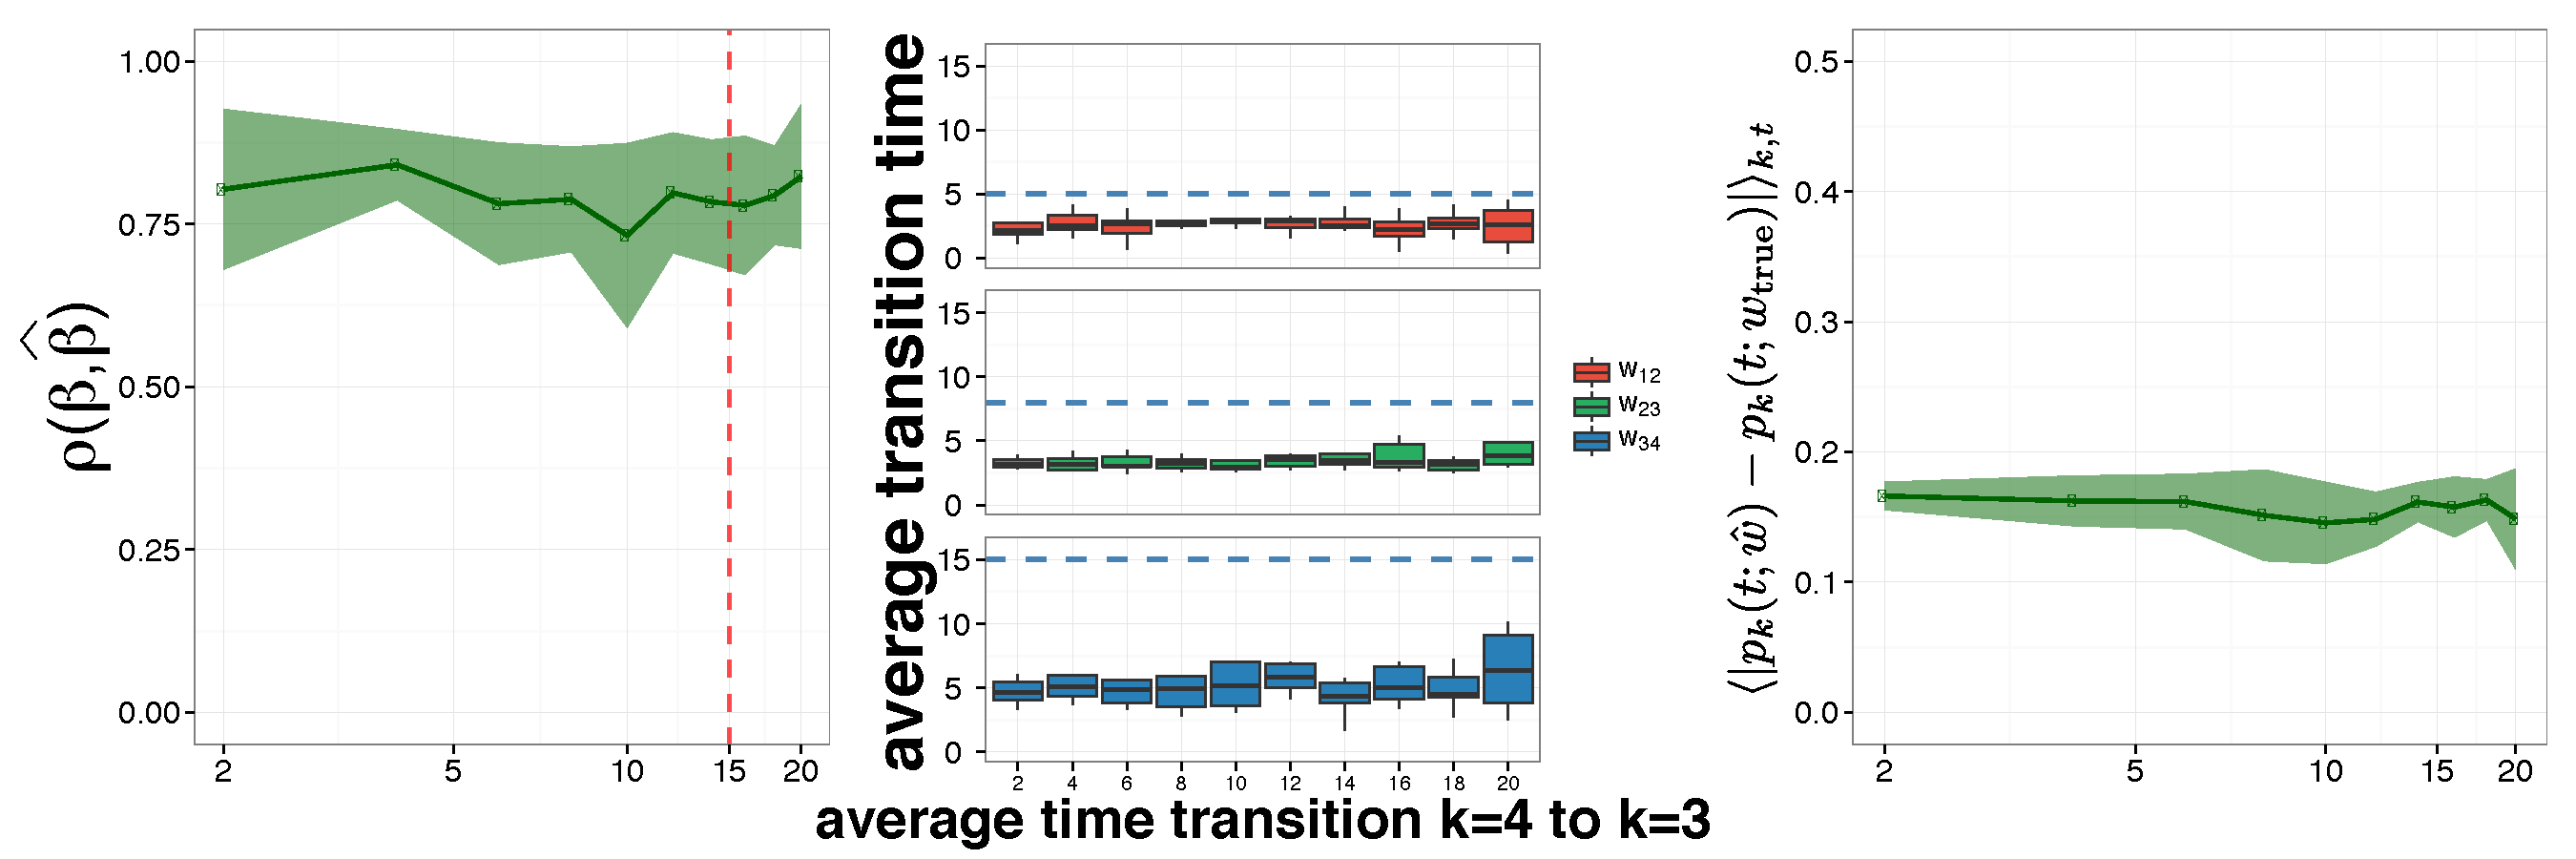
\includegraphics[width=1\textwidth]{pics/back-trans.pdf}
  \caption{Simulation study. To test the affect of back transition on the estimation, we simulate trajectories with back transition at $k=4$ with different transition times. In the left panel we plot the average correlation for $10$ independent runs, between true and estimated $\beta_{kj}$ parameters for different average time for the back transition as a solid line. The shaded area shows the standard deviation. The vertical dashed red line shows the average forward transition time for $k=3$. The middle panel shows boxplots for the average transition rate estimated from the model for a system with $K=4$ and only forward transitions. The right panel shows the mean differences between estimated and true probabilities averaged over $10$ trajectories as a solid line and the shaded area represents the standard deviation.}
    \label{fig:back}
\end{figure}


The second assumption we test is the inclusion of back transitions in the single cell. We simulate trajectories with back transition from $k=4$ to $k=3$; they are sampled from exponential distributions with different means. In Figure \ref{fig:back} we show comparisons between estimated and true values of parameters as a function of the average back transition time from state $k=$. In the left panel we plot the average correlation for $10$ independent runs, between true and estimated $\beta_{kj}$ parameters as a solid line. The shaded area shows the standard deviation. The vertical dashed red line shows the average forward transition time for $k=3$. The middle panel shows boxplots for the average transition rate estimated from the model for a system with $K=4$ and only forward transitions. The right panel shows the mean differences between estimated and true probabilities averaged over $10$ trajectories as a solid line and the shaded area represents the standard deviation.

\paragraph{Markovian assumption}
\label{sec:stud-t-distr}


\begin{figure}
  \centering 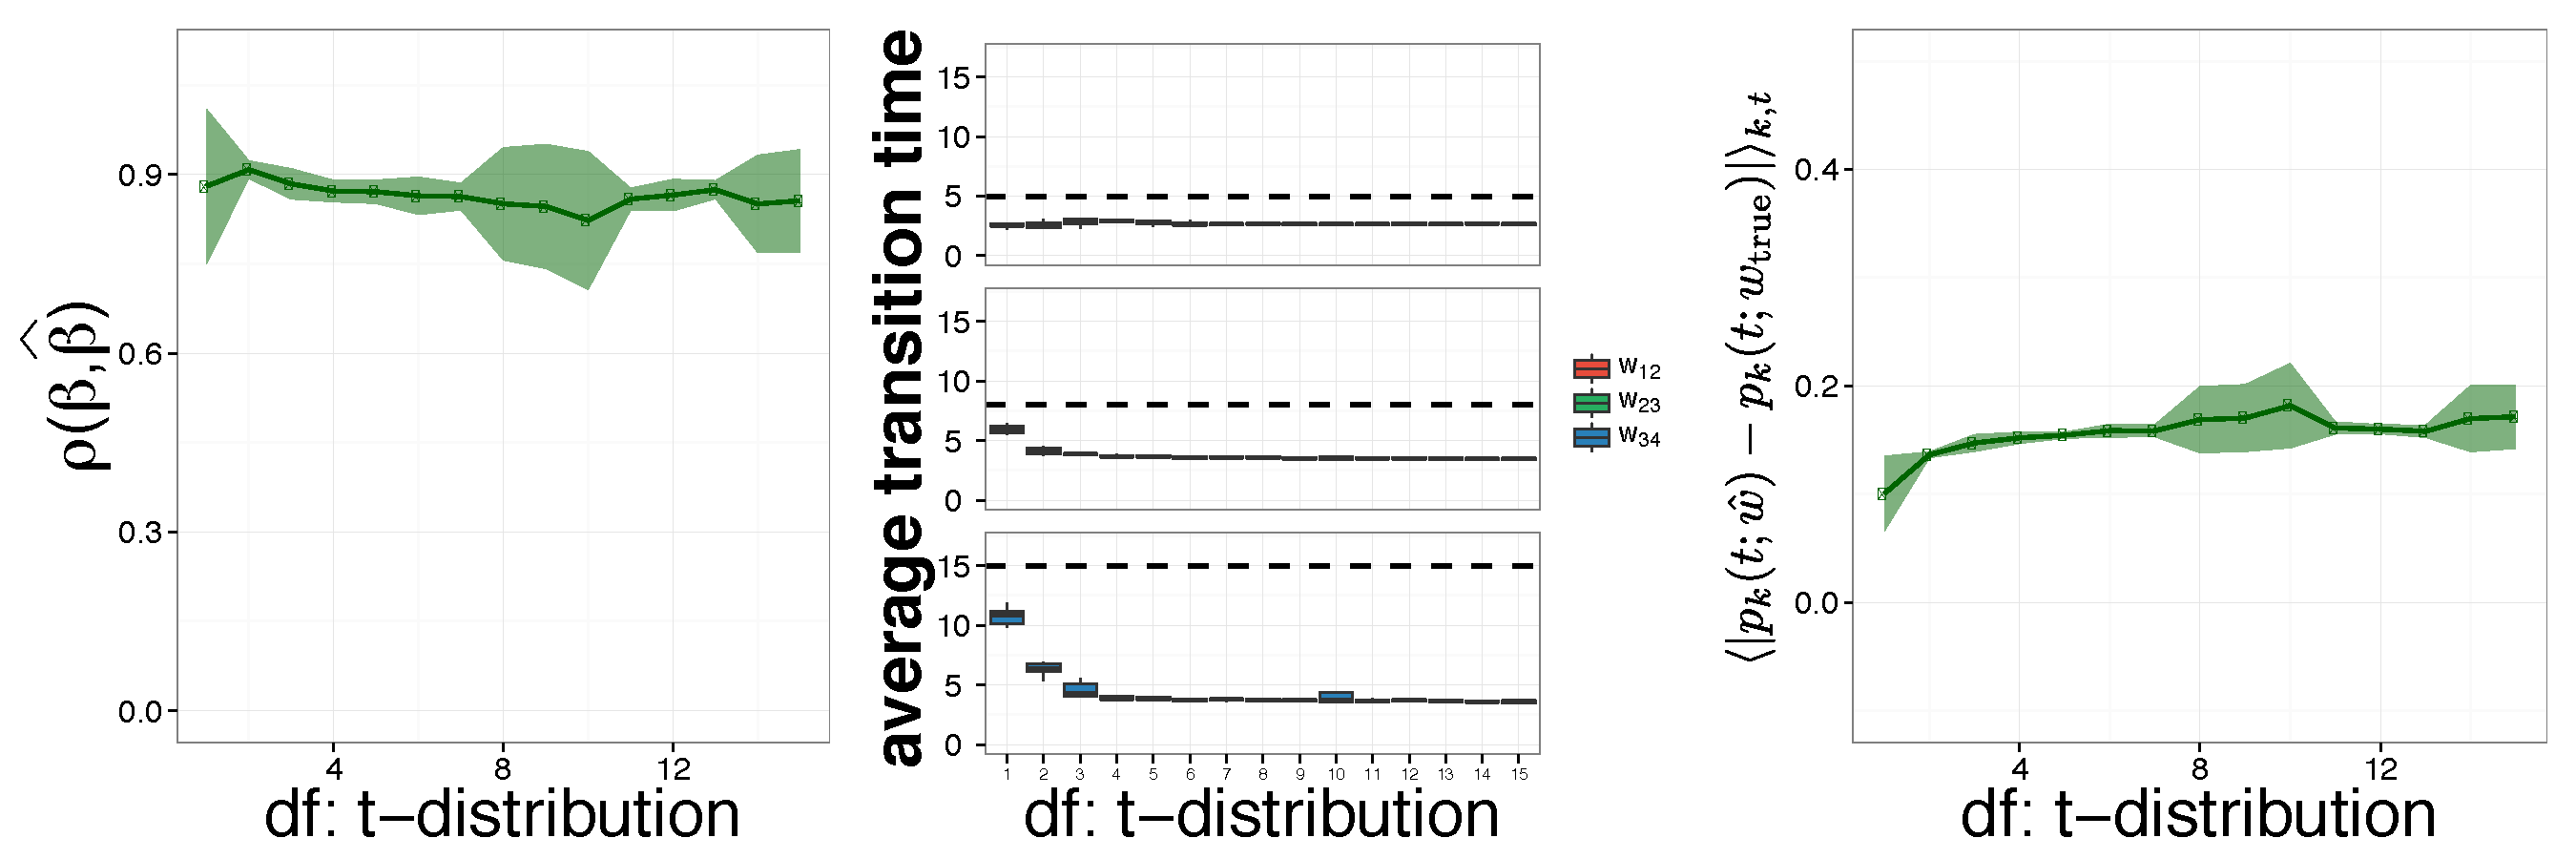
\includegraphics[width=1\textwidth]{pics/student-t.pdf}
  \caption{Simulation study. We simulate from a non-Markovian system, one where average transition rates are heavy tailed. Here we sample from a truncated Student t-distribution using the \emph{tmvtnorm} package in R. It is truncated at zero since transition rates are always positive. The transition rates are sampled to have means $(1/5, 1/8, 1/15)$ and we vary the degrees of freedom $df$ parameter in the package used. In the left panel we show the average correlation between true and estimated $\beta_{kj}$, the mean is shown as a solid line and the standard deviation as a shaded area. The middle panel shows boxplots for the for the average transition time estimated from the model for a system with $K=4$ states. The right panel shows the mean differences between estimated and true state occupation probabilities averaged over $10$ trajectories as a solid line and the shaded area represents the standard deviation.}
\label{fig:student}
\end{figure}


Finally in this section we investigate the latent Markov process and consider a case where jumps are non-Markovian. We want to consider the more realistic case that the transition time is fat tailed; therefore we choose a truncated Student t-distribution with a variety since transition rates are positive. We sample using the \emph{tmvtnorm} package in R with degrees of freedom, $df$, as the varied parameter. We perform the simulation as before, but sample transition rates from the t-distribution with means $(1/5, 1/8, 1/15)$ and consider a range of $df$ parameters in \emph{tmvtnorm}. The results are shown in Figure \ref{fig:student}; the left panel shows the mean correlation between true and estimated $\beta_{kj}$ as a solid line and the shaded area constrains the standard deviation. The middle panel shows boxplots for the average transition rate estimated from the model for a system with $K=4$ and only forward transitions. The right panel shows the mean differences between estimated and true probabilities averaged over $10$ trajectories as a solid line and the shaded area represents the standard deviation.


\subsection{Large scale simulation}
\label{sec:large-scale-model}

\begin{figure}
  \centering
  \subfigure[k-means clustering]{
    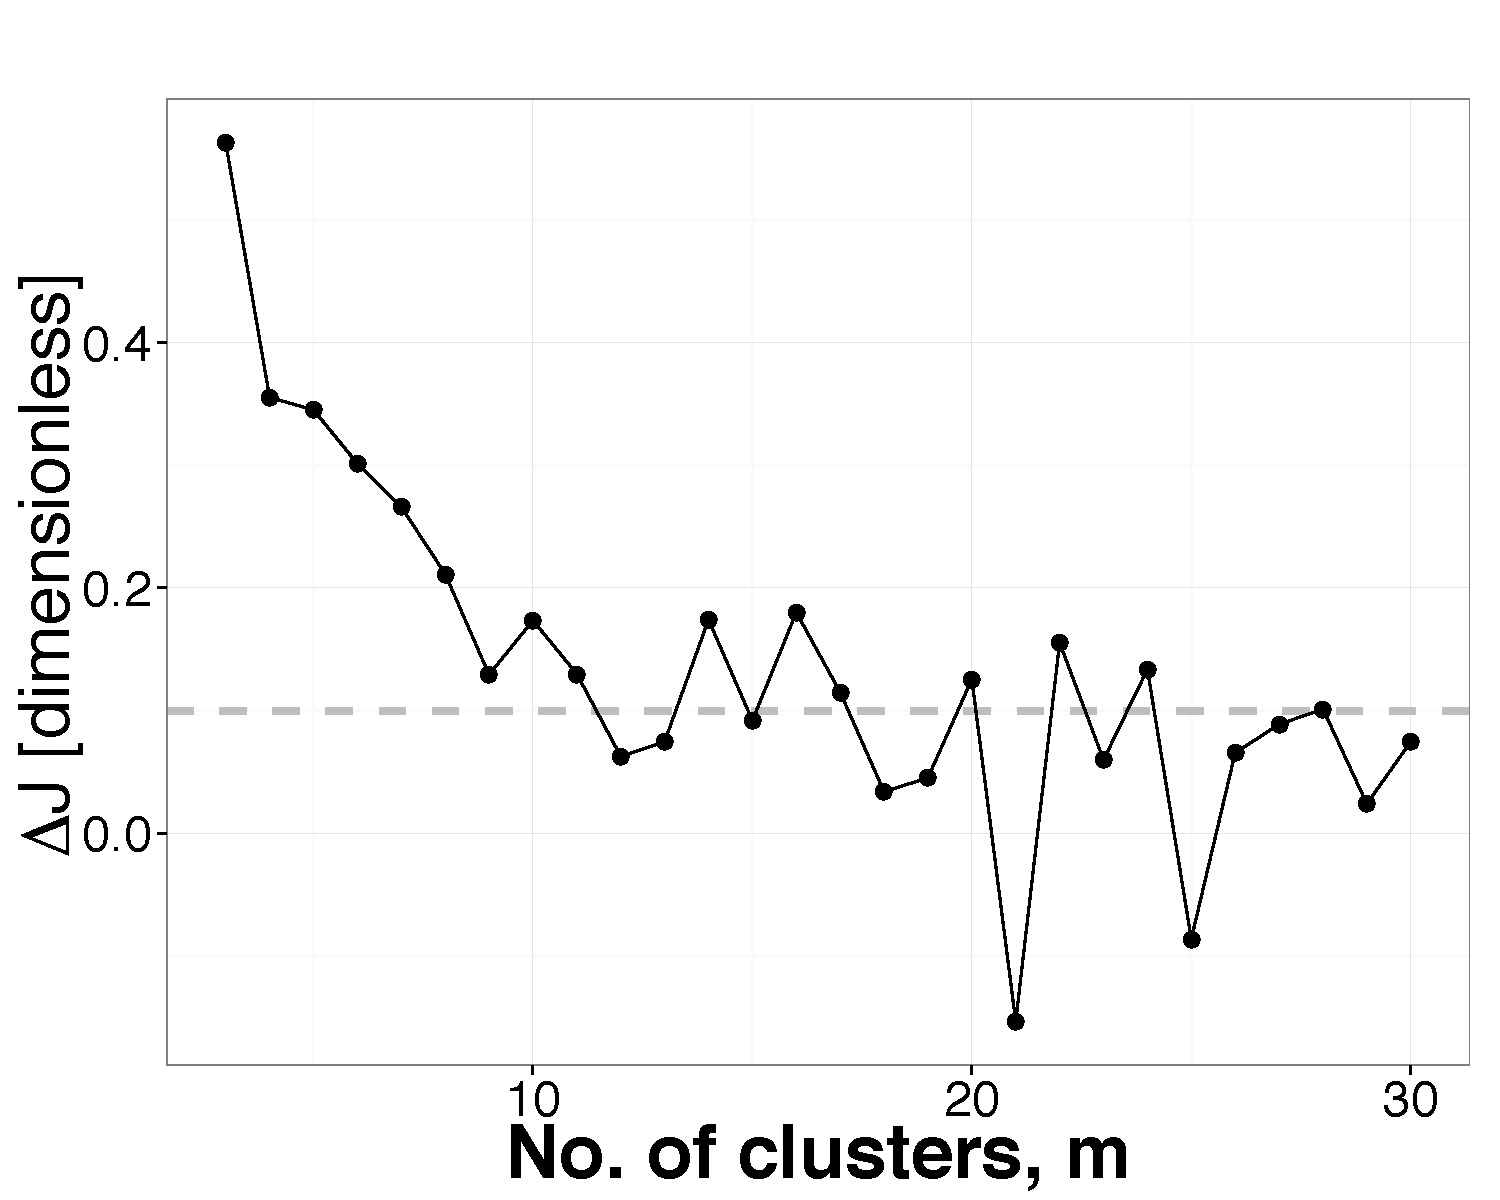
\includegraphics[width=0.47\textwidth]{pics/kmeans-sim.pdf}
    \label{fig:lrg-sim-clust-J}
  }
  \subfigure[transition rates]{
    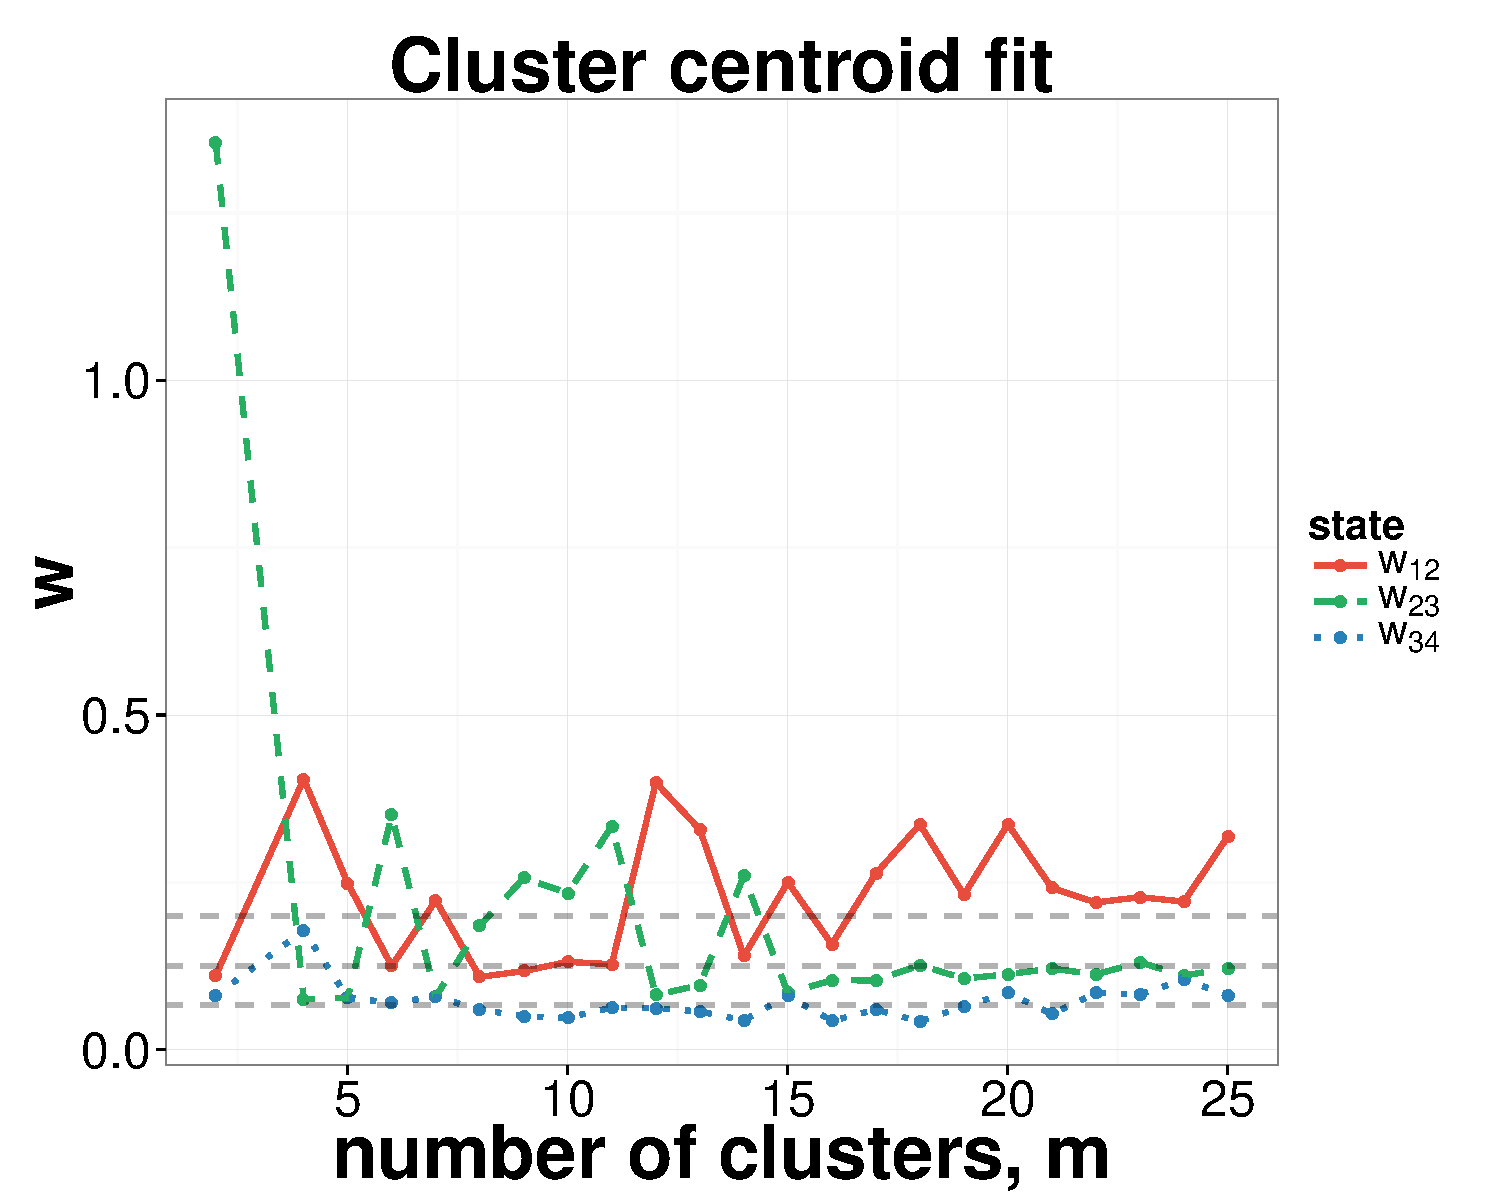
\includegraphics[width=0.47\textwidth]{pics/w_m_clust.pdf}
    \label{fig:lrg-sim-trans}
  }
  \caption{Large scale simulation study. Results from clustering. \subref{fig:lrg-sim-clust-J} Initial step in the estimation pipeline is use k-means clustering for $p=120$ genes. The plot shows relative change in the k-means objective function as a function of the number of cluster: $\Delta J(m) = 1 - J(m) / J(m - 1)$. We choose the optimum number of clusters $\hat{m}$ such that $\Delta J(m - 1) < 0.1$; here $\hat{m} = 13$. For larger $m$, $J(m)$ is small therefore relative changes have large fluctuations. \subref{fig:lrg-sim-trans} Estimated transition rates as a function of the number of cluster. Horizontal dashed lines show true values. After large initial fluctuations the transition rates fluctuate around the true value.}
  \label{fig:lrg-sim-clust}
\end{figure}


Lastly we want to check how well the two-step estimation pipeline outlined in Section \ref{sec:estim-pipe} works applied to simulated data. We simulate $p=120$ genes as described above with $K=4$ states. To mirror real data where genes are on different scales, we sample $12$ scale parameters $tau$. To get to $p=120$ genes we sample from all scale parameter $10$ sets of $\beta$ values. All other parameters are as set out in Section \ref{sec:sim-study}. We follow the procedure set out above and start by clustering simulated trajectories into $m$ clusters. Then we estimated transition rates $\mathbf{w}$ from cluster centroids and keep them fixed for the second step. Next we use these transition rates and estimate expression signatures $\beta_j$ independently for each gene $j$.




\subsection{Number of states}
\label{sec:number-states-res}

\begin{figure}
  \centering
  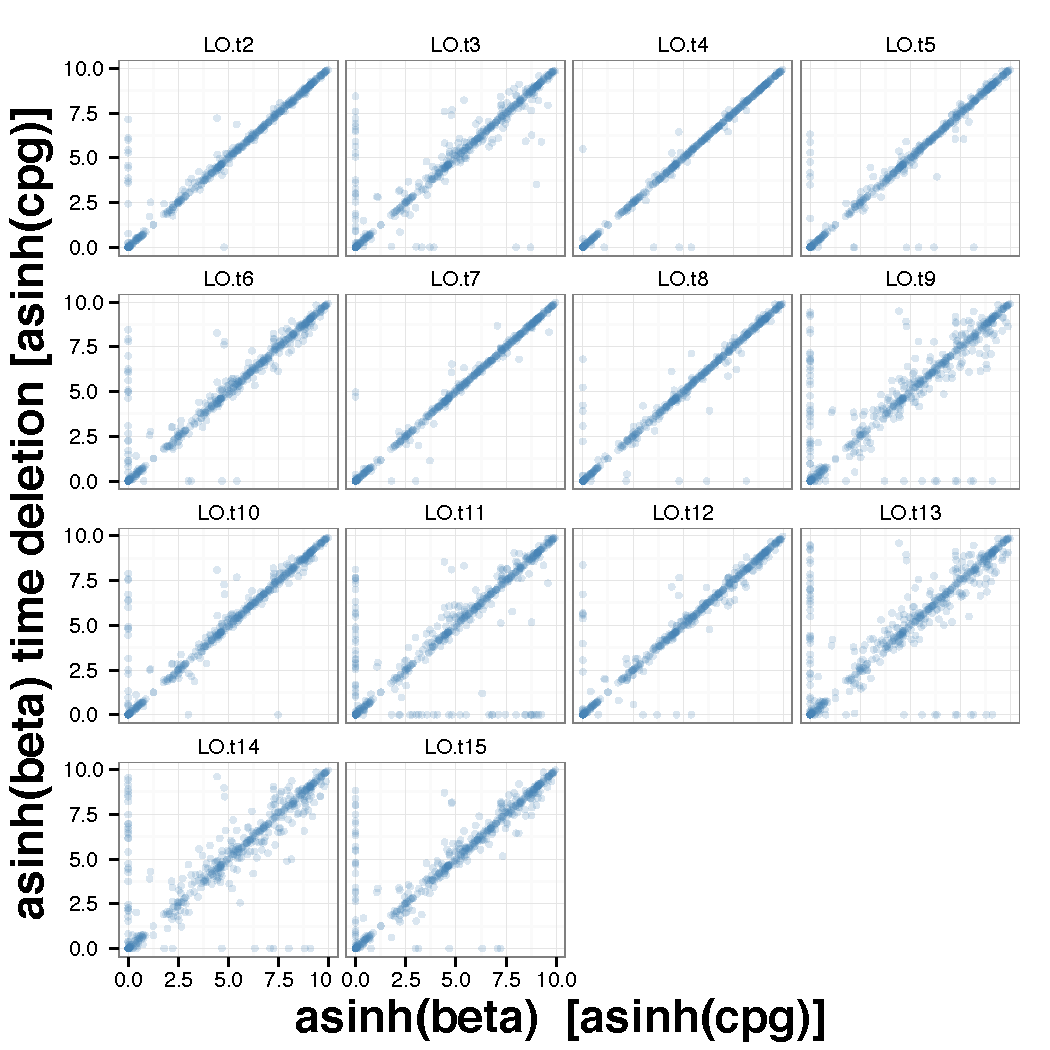
\includegraphics[width=0.6\textwidth]{pics/no-pen-sim.pdf}
  \caption{Large scale simulation. Stability of estimated expression signatures under time point deletion to determine need for $\ell_1$ penalization. We conclude that estimated parameters are stable therefore there is no need for a penalty.}
  \label{fig:lrg-sim-stab-l1}
\end{figure}

\begin{figure}
  \centering
  \subfigure[Number of states]{
    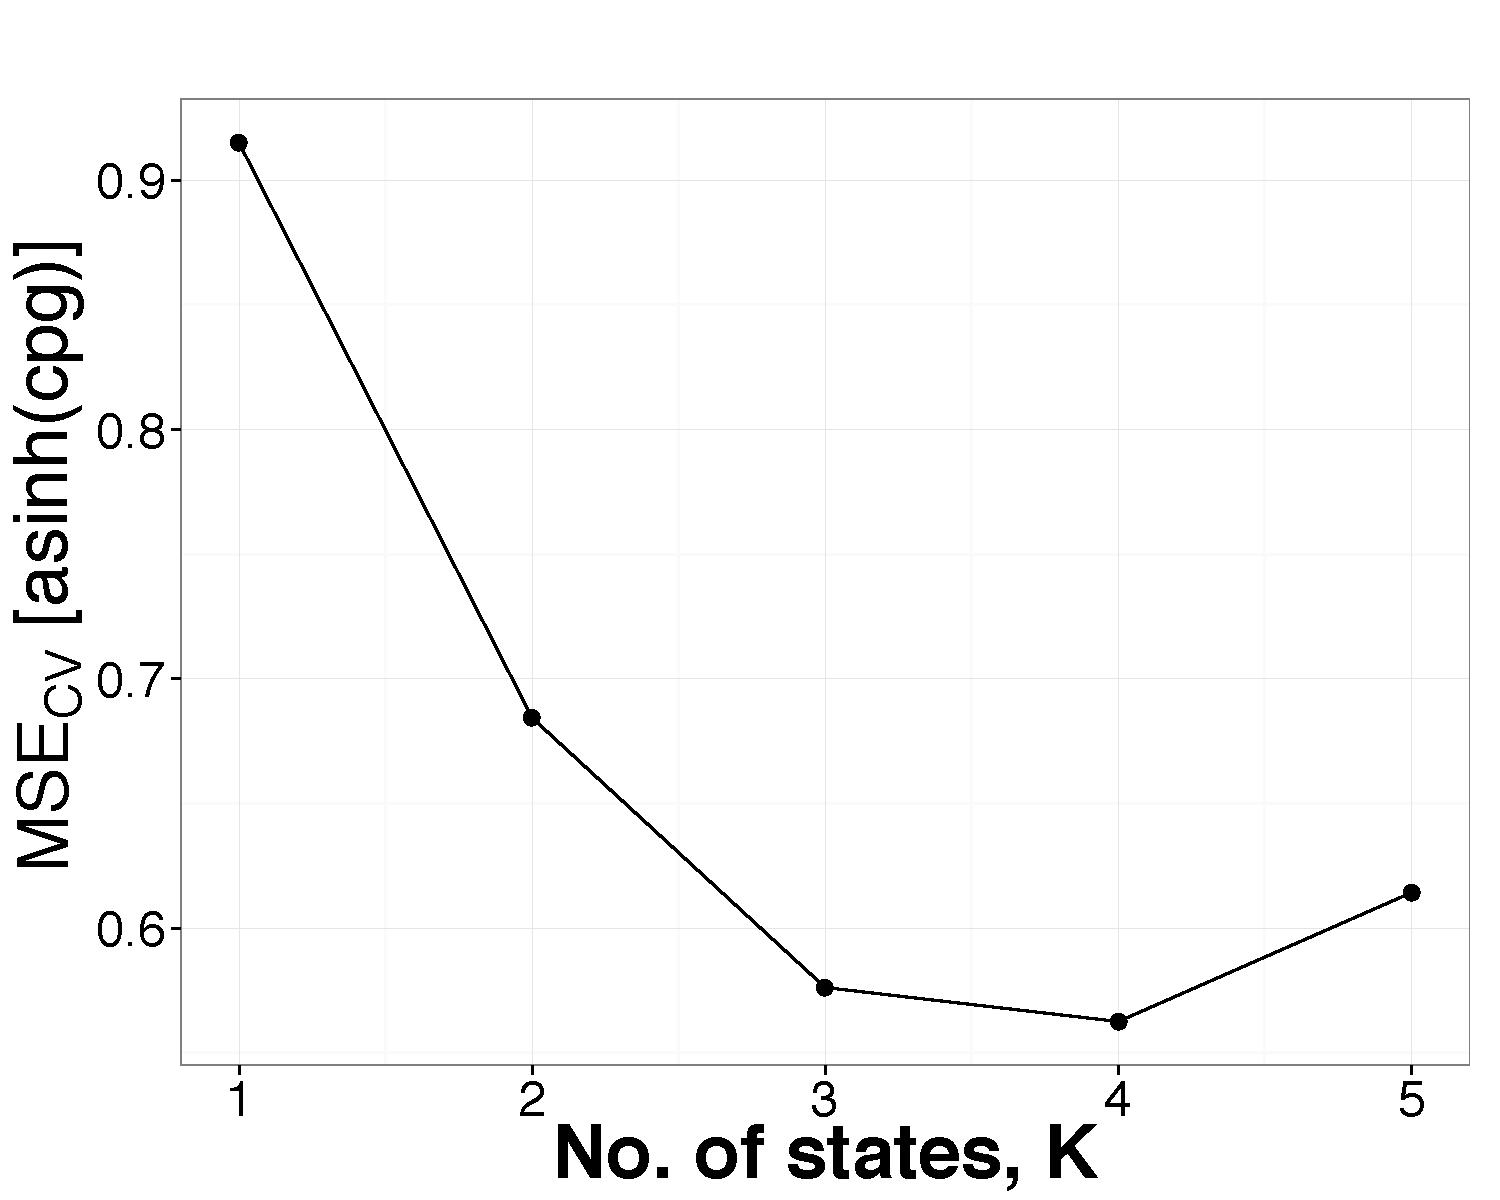
\includegraphics[width=0.46\textwidth]{pics/loocv-sim.pdf}
    \label{fig:lrg-sim-k}
      }
  \subfigure[Stability number of clusters]{
    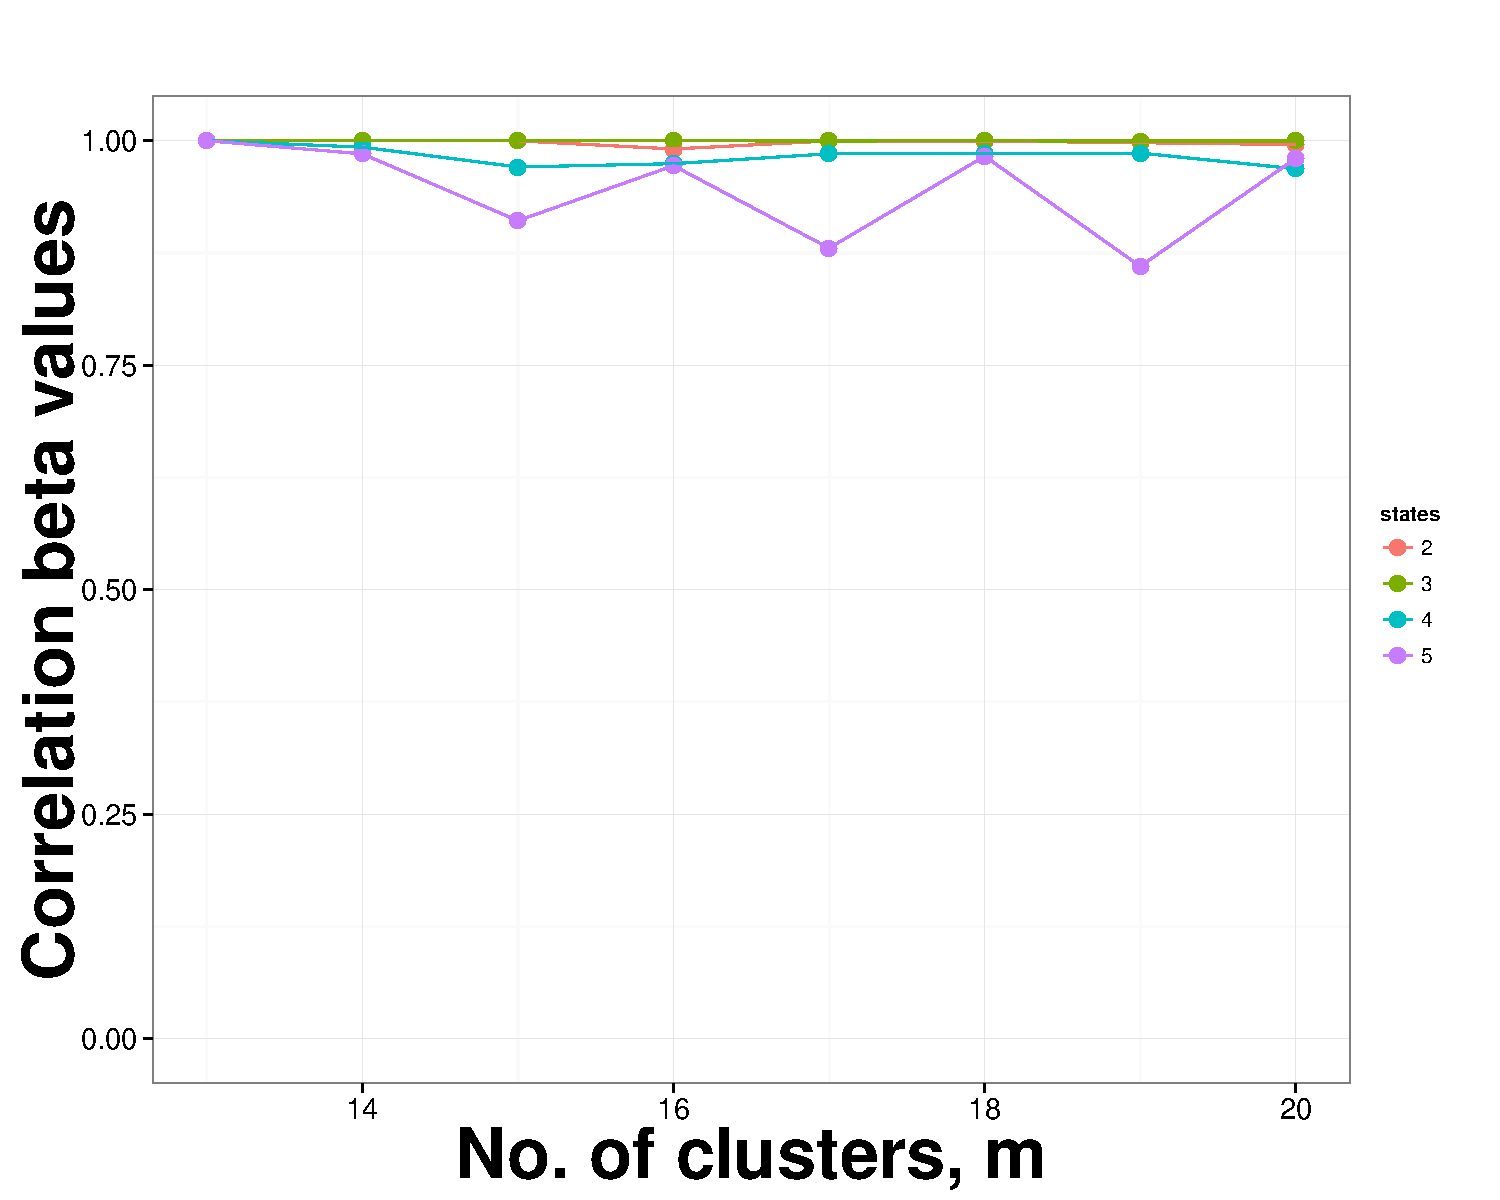
\includegraphics[width=0.46\textwidth]{pics/stab-m-sim.pdf}
    \label{fig:lrg-sim-mStab}
  }
  \subfigure[Permuted time points]{
    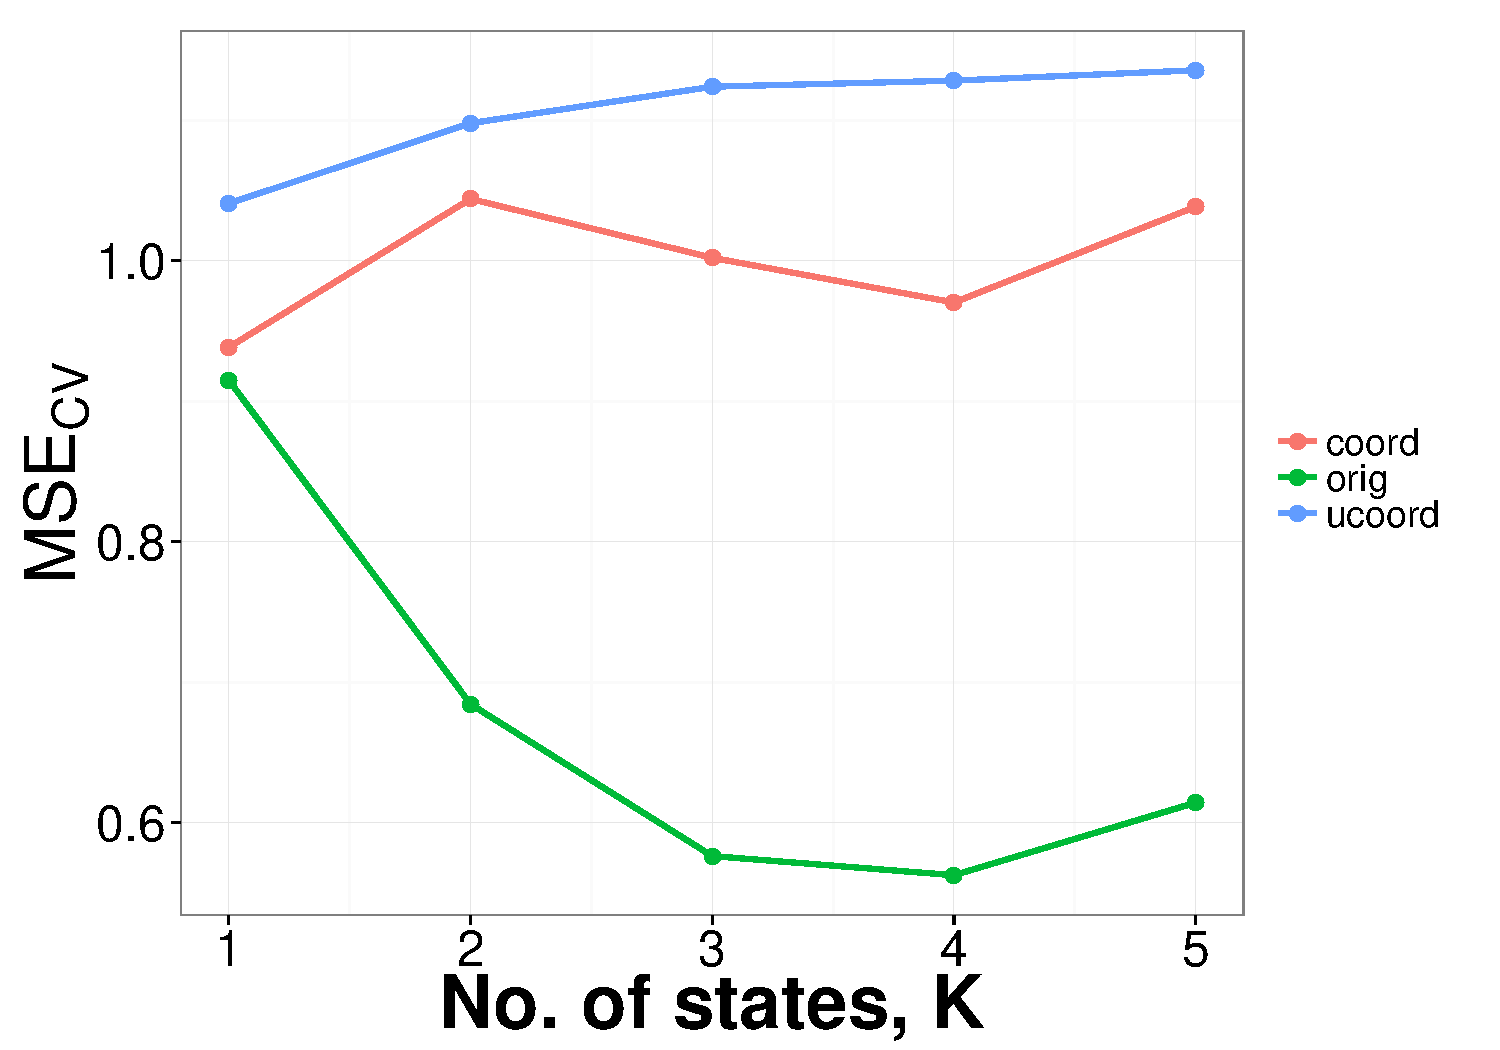
\includegraphics[width=0.48\textwidth]{pics/sim_permute.pdf}
    \label{fig:larg-sim-permute}
  }
  \caption{Large scale simulation. Simulation performed for $p=150$ genes, $15$ time points and $K=4$. Figures summarise results obtained from applying the estimation pipeline (see Section \ref{sec:estim-pipe}) to the simulated data. \subref{fig:lrg-sim-k} $\mathrm{MSE_{CV}}$ score to determine optimal number of states in the model, the minimum is at $K = 4$. \subref{fig:lrg-sim-mStab} Test to determine stability under perturbation of number of clusters $\hat{m}$. Estimation is stable therefore the choice of parameters is reasonable. \subref{fig:larg-sim-permute} To determine dependence on structure of data we perform a permutation test, first by permuting time-points of all trajectories in a coordinated fashion and then by permuting trajectories independently. The $\mathrm{MSE_{CV}}$ score for permuted data is significantly higher for all $K$ other than $K=1$ and data permuted in a coordinated fashion perform better than independently permuted data.}
  \label{fig:lrg-sim-k-m}
\end{figure}


Applying the first step we cluster the simulated data using a k-means clustering algorithm. We use the relative decrease in the objective function $\Delta J(m)$ to determine the number of clusters and vary $m$ in the range $[2, 30]$, see Figure \ref{fig:lrg-sim-clust}. The relative decrease is smaller than $0.1$ for $m=12$ therefore we choose $\hat{m} = 13$. Note that for larger $m$ the objective function $J(m)$ is small and we observe that $\Delta J(m)$ has large fluctuations due to slight deviations in the objective function. Then we test if for this set of data penalisation is necessary using stability of estimated gene expression signatures under deletion of time points. Figure \ref{fig:lrg-sim-stab-l1} shows that for all deletions estimated parameters are stable, therefore we conclude that there is no need for a penalty term. Then we perform a model selection step to determine the number of states $K$ of the latent Markov chain. We compute the $\mathrm{MSE_{CV}}$ score for $K=\lbrace 2, \ldots, 5 \rbrace$ states, see Figure \ref{fig:lrg-sim-k}; we see a clear minimum for $K=4$ which is also the correct number of states. In the final step of the pipeline we perform a post-estimation stability test to ensure the number of clusters chosen is not too small (see Section \ref{sec:estim-pipe}). We compute the correlation for expression parameters estimated with increasing number of clusters, see Figure \ref{fig:lrg-sim-mStab}. We carry out this test for all models $K = \lbrace 2 \ldots 5\rbrace $ and the estimated parameters are stable therefore we conclude that the choice of $\hat{m}$ was a reasonable choice. 

A question that arises from these results is to what extent they are indicative of estimation or if states are only estimated because the model assumes there are states in data. One good way of addressing this question is to permute data and compare  $\mathrm{MSE_{CV}}$ estimated for permuted data and the original data. Here we distinguish between two ways of permuting data: first we perform a coordinated permutation where all simulated trajectories are permuted in the same way. Then we perform a permutation for each trajectory independently. In Figure \ref{fig:larg-sim-permute} we show the results and we can see that with both types of permutations the $\mathrm{MSE_{CV}}$ values are significantly larger than the original data set.


\subsubsection{Estimated parameters}
\label{sec:transition-rates}

One of the strengths of using simulated data is that we can compare estimated and true parameters. Figure \ref{fig:lrg-sim-scatter-b} shows a scatter plot of estimated $\beta$ parameters against their true values used in the simulation. The parameters are in general well estimated with a Pearson correlation of $0.95$; despite that as the plot shows in certain cases the true value of $\beta$ is exactly zero but estimates are non-zero. 

\begin{figure}[!h]
  \centering
  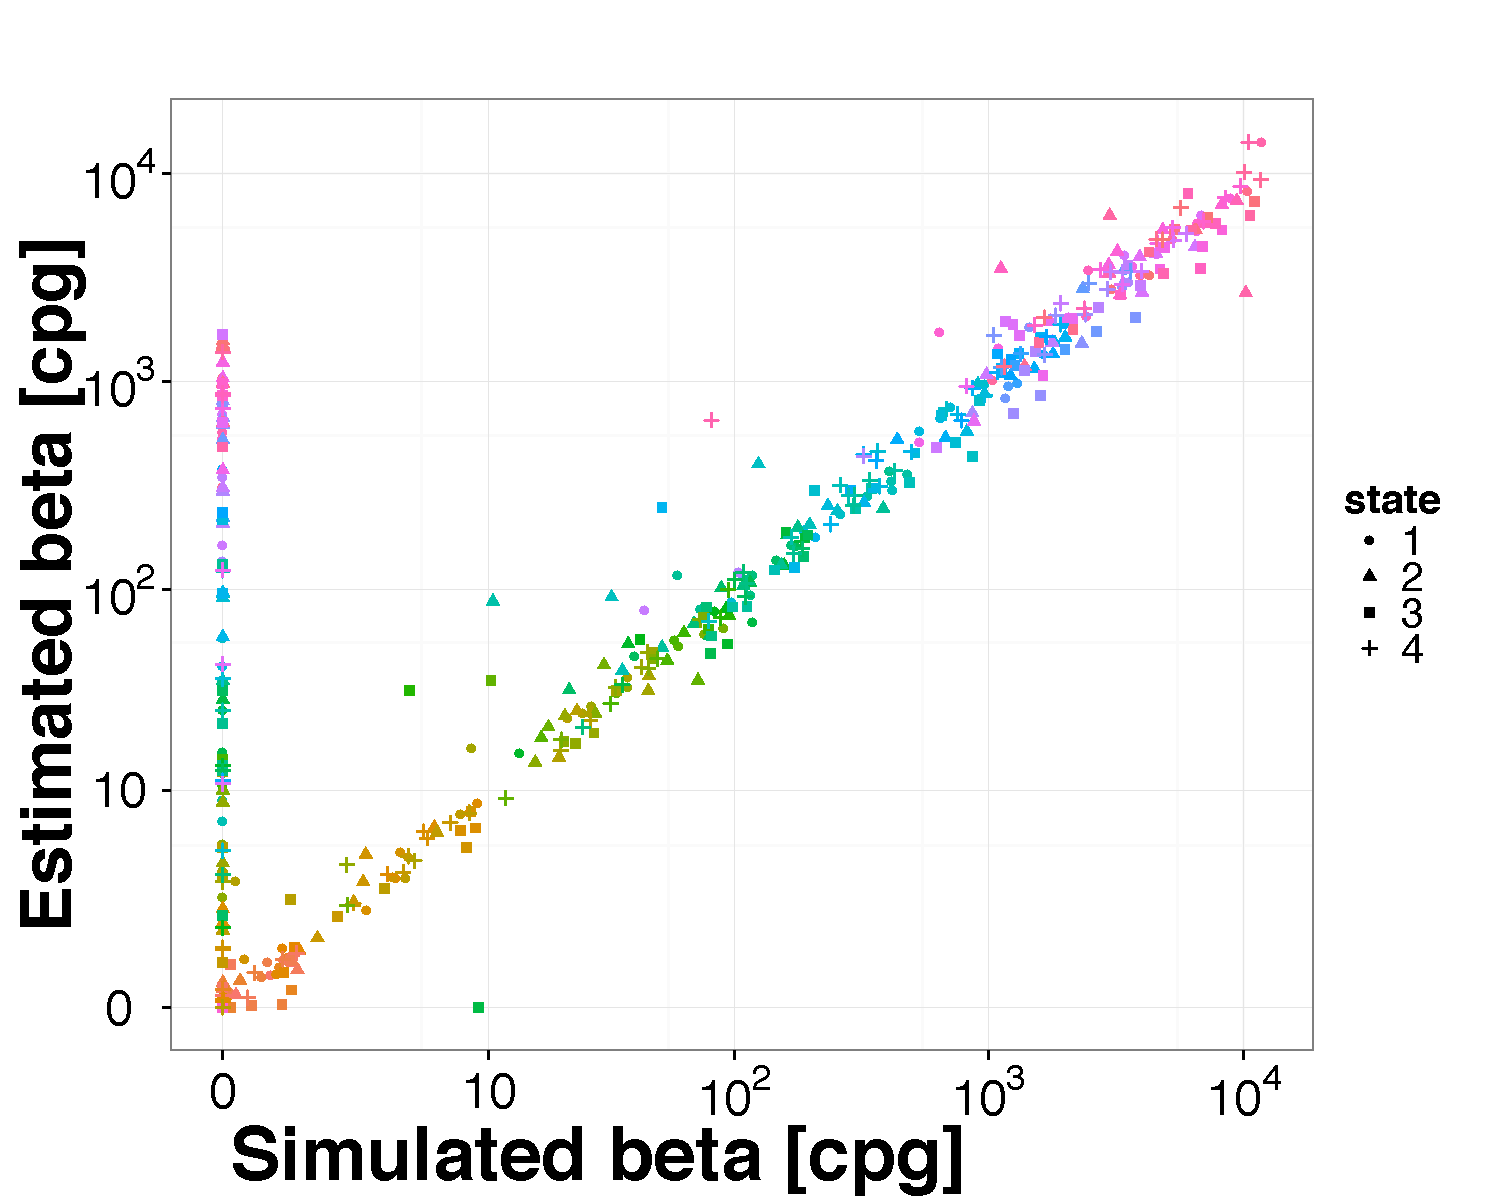
\includegraphics[width=0.8\textwidth]{pics/beta-sim.pdf}
  \caption{Large scale simulation. Estimated gene expression signatures scattered against their true values. }
  \label{fig:lrg-sim-scatter-b}
\end{figure}

The first clustering step we take is crucial and has a considerable affect on parameter estimation of transition rates. Hence it is valuable to delve a bit deeper into the first estimation step and its sensitivity to the number of clusters. Figure \ref{fig:lrg-sim-mStab} shows that estimates expression signatures are very stable when increasing number of clusters. Figure \ref{fig:lrg-sim-trans} shows the three transition rates for a model with $K=4$ as a function of $m$. The horizontal dashed lines in the plot show true transition rates. We observe that estimated transition rates strongly fluctuate for small $m$ and with increasing number of clusters fluctuations decrease. are highly sensitive to changes in $m$,

\section{Discussion}
\label{sec:discussion}

We present an extension to previous work with a detailed description of the model including its assumptions, an unbiased estimation pipeline and simulation based tests to investigate STAMM recently proposed in \cite{Armond:2013}. To address concerns about practical application we have made computation more efficient including the use of parallelisation which due the two-step estimation process allows much larger efficiency; the exploration of model behaviour under violation of underlying assumptions; and an extension to allow for application to RNA-seq data though more on that in Chapter \ref{cha:oncog-transf}.


% sims and identifaibility

Establishing investigating identifiability in a latent stochastic model aggregate over single-cells is highly non-trivial. Some relevant literature exists \citep{Kalbfleisch:1983vd, Kalbfleisch:1984wz, Kalbfleisch:1985tw}), but it is applied to panel data or the latent stochastic model is in discrete time. Identifiability results that can directly be applied to STAMM do not exist yet.  Therefore we present empirical results using single-cell simulations and show that true parameters used during simulation can be identified. However it is important to understand the explore restrictions on Markov chain topology. Especially if there is potential for allowing more complex topology (e.g. including branches or back transitions) by including additional single cell data. This would allow for precise experimental design in applications to ensure more details can be determined about transformation processes.
  
To allow for efficient estimation and to ensure identifiability of model parameters a number of simplifying assumptions are made in STAMM. Of course these assumptions do not hold in real biological systems. To investigate capabilities and limits of STAMM we simulated data by braking these assumptions in turn. In summary, we find the model relatively robust under violations of underlying assumptions, but especially transition rates under strong violations of the assumptions are estimated badly. This leads to the conclusion that even though state-specific gene expression signatures are often well estimated they should serve as hypothesis to be confirmed by experiment.

% future prospects, how can be used to design experiments

STAMM is versatile in its application as it can be used for a broad range of transition processes and data types. Two data types we investigate in this thesis are microarray data and RNA-seq data but it can also applied to transcript, protein and epigenetic time course assays. New development of cheaper bulk assays means it is a feasible first step to study a transforming biological system. STAMM could be used to identify a subset of genes important in transformation; to pinpoint cell surface markers that distinguish states facilitating a single cell separation; or discovery of transition to allow for targeted single-cell experiments. Using multiple types of data in iterative stages would allow for a step by step improvement in information gathered about the system. For instance once transition rates are known estimation of expression signatures is much more precise and vice versa. In future it would also be interesting to relax some of the assumptions made and extend them model.


%%% Local Variables:
%%% TeX-master: "warwickthesis"
%%% End:
